%!TEX root =  ../main.tex

\chapterimage{Nasir-al_molk_-1} 
\mychapter{Transformations}{transformations}

More complicated things can happen to functions, not the least of which is that they can be nested, 
like Russian dolls.  It is also possible for the $x$ and $y$ of our graphs to be defined by some
other variable, call the parameter.  That skill-set will then unable us to see which functions can
be ``undone'', and which cannot be (or at least not perfectly).  It is also possible 
to analyze the reciprocal of a function.   We will also consider what happens when the input and/or
output of a function is a distance, i.e. absolute value.

\inlinefig{Inner_Circle}{Russian or Matryoshka dolls are famous for being \emph{nested}.}
% https://www.flickr.com/photos/jronaldlee/5566380424

\newpage
\chapterminitoc

%							4 - 1
\newpage
\invisiblesection{Absolute}
\subsection{I'm Batman}
Word doc
\newpage
%!TEX root =  ../main.tex

\subsection{Inside and Outside}

\objective{Graph and apply absolute value transformation}


\index{Absolute Value!Transformation}
Consider what applying absolute value does as a \emph{transformation}.
First of all, what would $y=|f(x)|$ do?  Obviously, this will prevent $y$ from ever being negative.
But what happens to those negative segments of the function?  They --- and they alone ---
are reflected over the $x$-axis.  This creates cusps at every turn, moments that will
be un-differentiable.

What if we try $f(|x|)$?  This will cause negative inputs to receive the output as if they were
positive.  Graphically, this means the left-half of our graph will be the mirror image of the
right half.

\index{Absolute Value!of motion, terms}
\subsection{Distance, Velocity, Jerk}
Absolute value was invented to describe distance.  The verbal question ``how far is $x_1$ 
from $x_2$?'' is best represented as $|x_1-x_2|$.  Typically, we have some function modeling 
\textbf{position} and then we contrast that position with something else, 
and are asking a question of  \textbf{distance}.  What would have to be true about 
some graph to leave it susceptible to change 
by the application of absolute values?  How can absolute value transformation produce
undifferentiable moments in a graph?

Another common function to deal with in physics is a speed graph.  This too can be negative,
which when converted to \textbf{velocity}, might make issues. Another source of difficulty
is when we disregard the sign of our input, effectively transforming into $f(|x|)$.  Thinking
graphically, how would the left side correspond to the right?  What kind of symmetry would
such a transformation enforce?  The derivative of speed is position.

Lastly, we will often consider acceleration.  Most processes effected by acceleration 
do not care if it is positive or negative (deceleration).  The absolute value of the 
acceleration is sometimes called  ``jerk'', though this term is not universally standardized.  
The derivative of acceleration is speed.

Studies have begun to come out about higher orders, functions whose derivative is acceleration 
(called snap, crackle, and pop), but these terms are so rarely needed that the names are trivial.
  

\newpage
\subsection{Exercises}
Word doc



%							4 - 2
\newpage
\section{Parametric}
\subsection{x, y, ... t?}
Word doc
\newpage
%!TEX root =  ../main.tex

\subsection{Separating $x$ and $y$}

\objective{Use parametric functions to determine a path and velocity}


Physics teaches us that it is often preferable to separate $x$ and $y$, and to
consider them both functions of $t$ and not one a function of the other.  This is 
typically done because gravity (which Einstein showed to be the same as 
acceleration, and hence is a quadratic equation) pull in one dimension, while
the others are simple linear equations.

Another benefit to parameterizing an equation, is that we also can \emph{when}
something happened.  So far, we have been differentiating $y$ with respect to 
$x$, but what if we want to know how quickly $y$ is changing over time?

\personfeature[0in]{\chapdir/pics/Maria_Gaetana_Agnesi_(1836).png}{Maria Gaetana Agnesi}{1718-1799}{was an Italian mathematician, philosopher, theologian and humanitarian. She was the first woman to write a mathematics handbook and the first woman appointed as a Mathematics Professor at a university.  The parametric curve $$y=\frac{8a^3}{x^2+4a^2}$$ (The Witch of Agnesi) is named after her.\href{https://en.wikipedia.org/wiki/Maria_Gaetana_Agnesi}{Wikipedia}}

\subsubsection{Parameter Domain}
Parameters (most often $t$) also have a domain.  In science, it is often quite
irrelevant to reference any of the variable before the experiment begins or
after it ends.  If an object is thrown on Earth, and we model its path with an
upside-down parabola, what happens before $t=0$ or after it hits the ground
is meaningless.  Parameters' domains provide a natural and intuitive way to
model this limited domain. 

\index{TI-8*!zoom standard}
Pay careful attention to the WINDOW on your TI-8*.  In RADIANS mode, the
default (i.e. ZOOM-STANDARD) parameter domain is $[0,2\pi]$.

\subsubsection{Eliminating the Parameter}
Sometimes, we still want to construct a typical equation from a parametric 
set.  This is called \textbf{eliminating the parameter}.  In chapter 10, we will
learn many trigonometric identities to remove sines and cosines of $t$, but in 
this section on algebraic functions, we will restrict ourselves to
\textbf{substitution} and \textbf{elimination}.

\subsubsection{Implicit Differentiation}\index{derivative!notation}
Until now, we have been solely using LeGrange notation for derivatives, e.g.
$y'$ (pronounced, ``$y$ prime'').  However, this isn't always helpful, especially
if we want to know what we have been differentiating with respect to.  Until now,
that hasn't mattered!  Now we might be looking for the differential of $y$ with 
respect to $x$, or with respect to $t$.

A differential is a measure of sensitivity to change.  How much does $y$ alter,
given minuscule nudges to $x$ (or $t$).  This differential can also be written with the
letter `d', and so ``the differential of $y$ over the differential of $x$'' can symbolized
as $\frac{dy}{dx}$.  It can also be used like a function, to say ``take the derivative with 
respect to $x$ of ...'', as in $\frac{d}{dx}\left( y\right)$.

This fractional way of writing derivatives is called \textbf{Leibniz's notation}, after
Gottfried Leibniz.  It helps show how we can find the derivative of a parametric equation.
If we seek $\frac{dy}{dx}$, that is equivalent to $\cfrac{\frac{dy}{dt}}{\frac{dx}{dt}}, \frac{dx}{dt}\ne
0$.

\index{derivative!higher order}
Derivatives of derivatives (called \textbf{higher order derivative}) were written 
with more tick-marks (e.g. $f''(x), f'''(x)$, etc.) or parenthetical numbers (e.g. $f^{(2)}(x),
f^{(3)}(x)$, etc.) in Lagrange notation.  For Leibnitz's, they get more complicated:
$\cfrac{d\left(\frac{d\left(\frac{dy}{dx}\right)}{dx}\right)}{dx} = 
\left(\frac{d}{dx}\right)^3y = \frac{d^3y}{dx^3}$.

~\vfill
%\newpage
\subsection{Exercises}
\noindent\makebox[\textwidth]{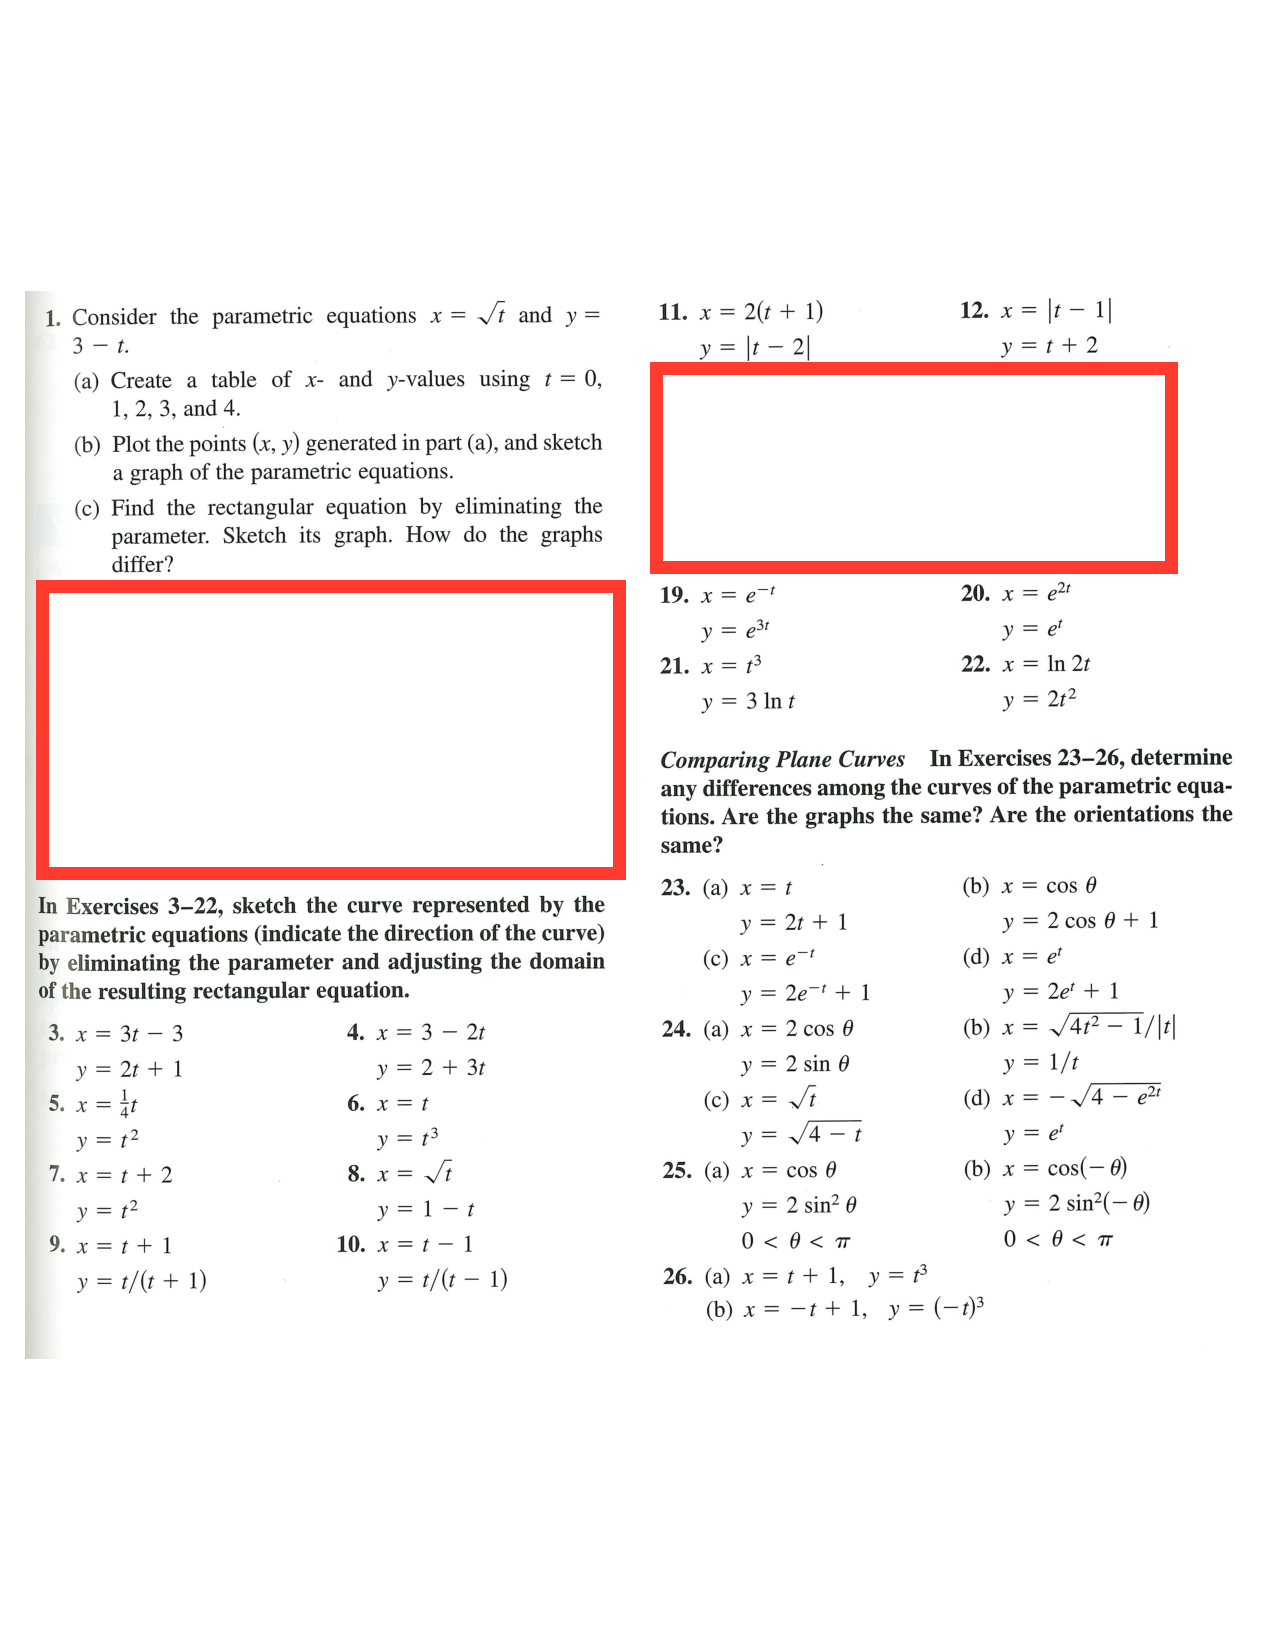
\includegraphics[width=\paperwidth]{ch04/0402xA.pdf}}
\newpage
\noindent\makebox[\textwidth]{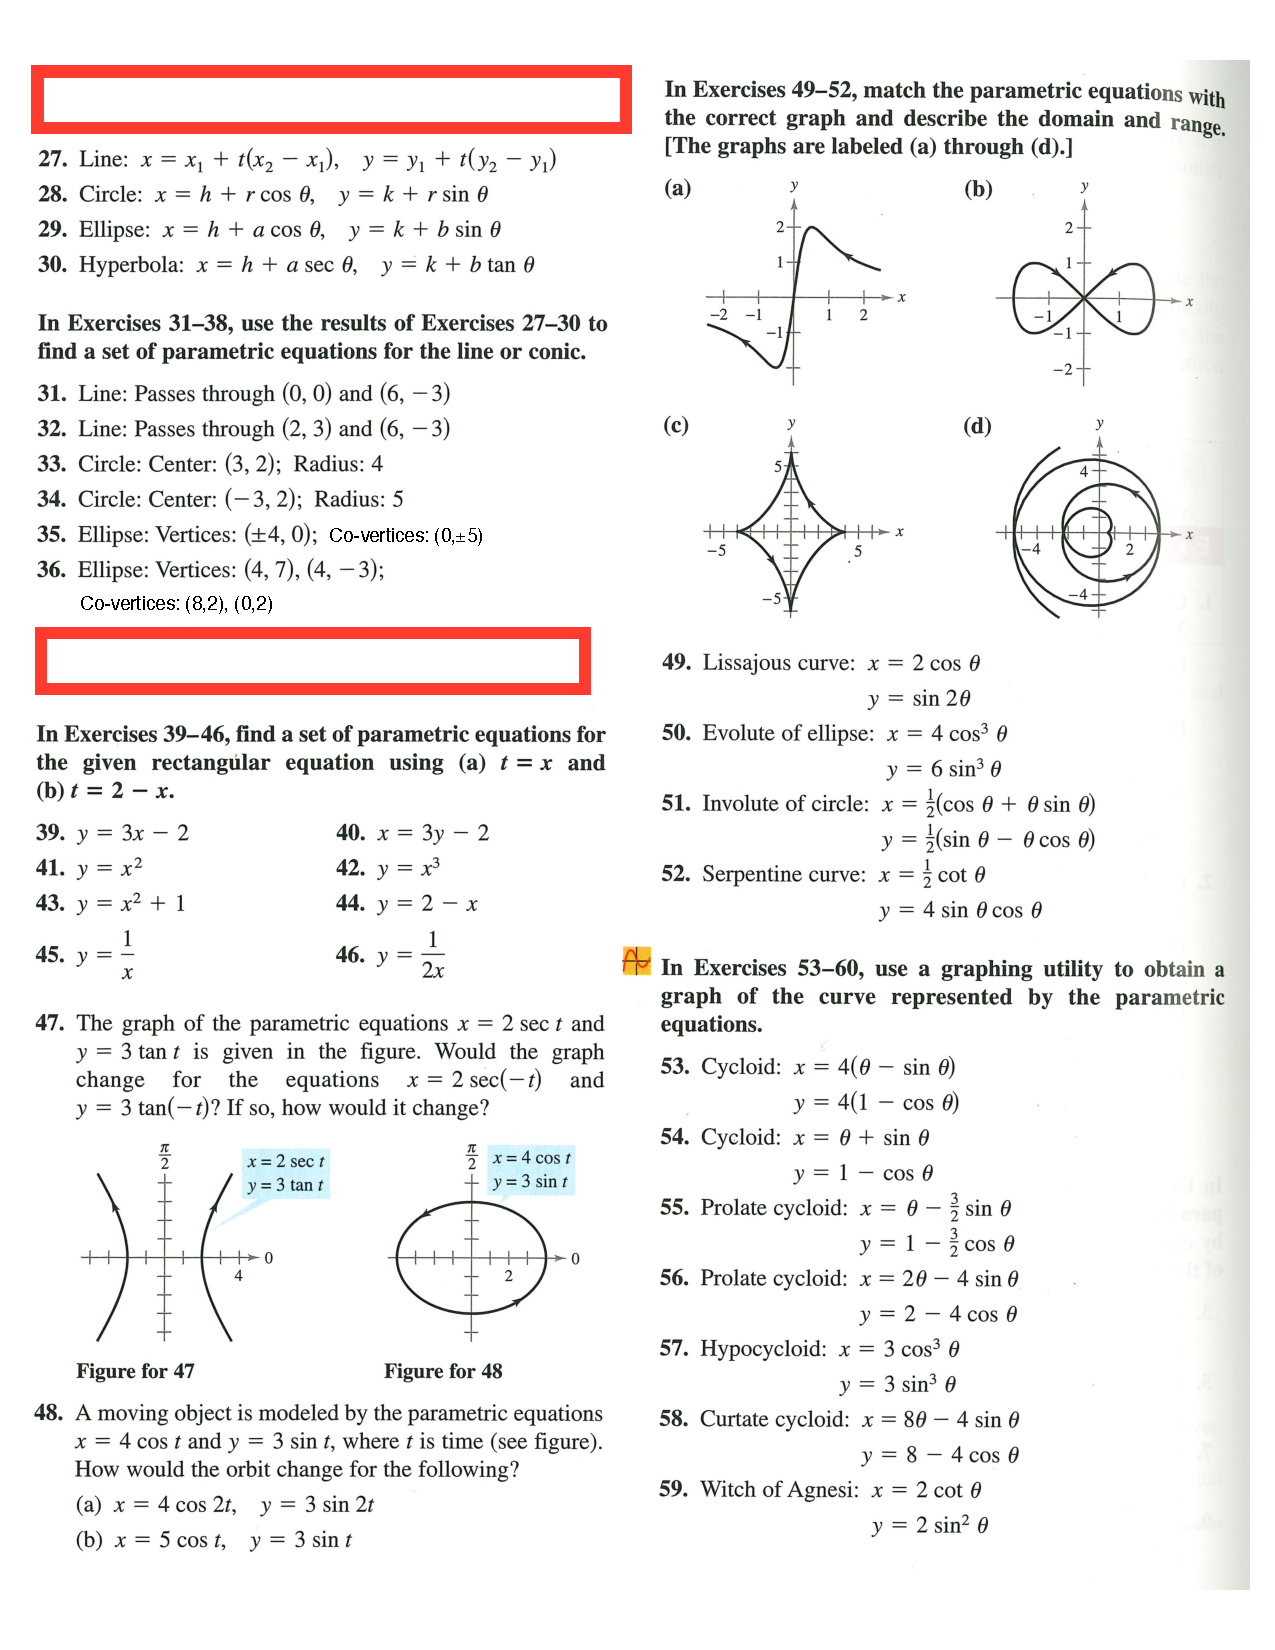
\includegraphics[width=\paperwidth]{ch04/0402xB.pdf}}
\newpage
\noindent\makebox[\textwidth]{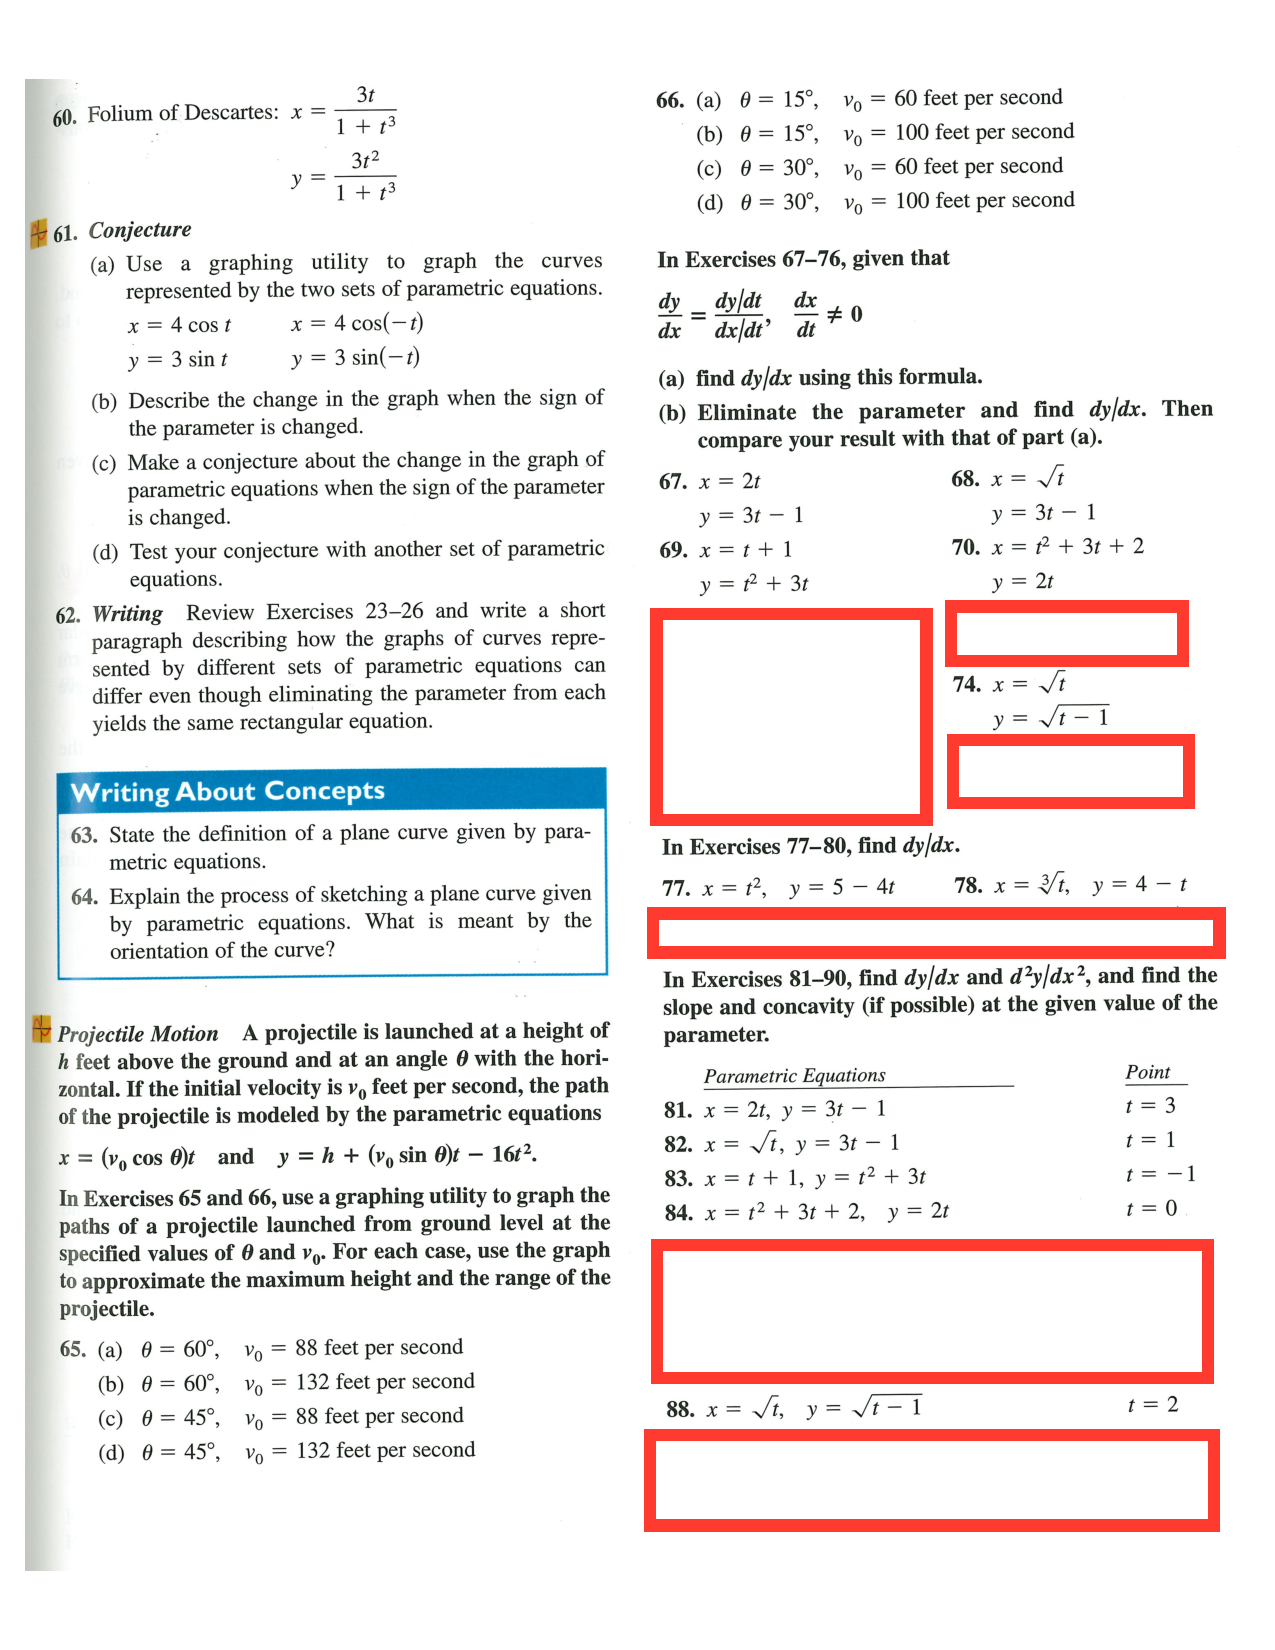
\includegraphics[width=\paperwidth]{ch04/0402xC.pdf}}
\newpage
\noindent\makebox[\textwidth]{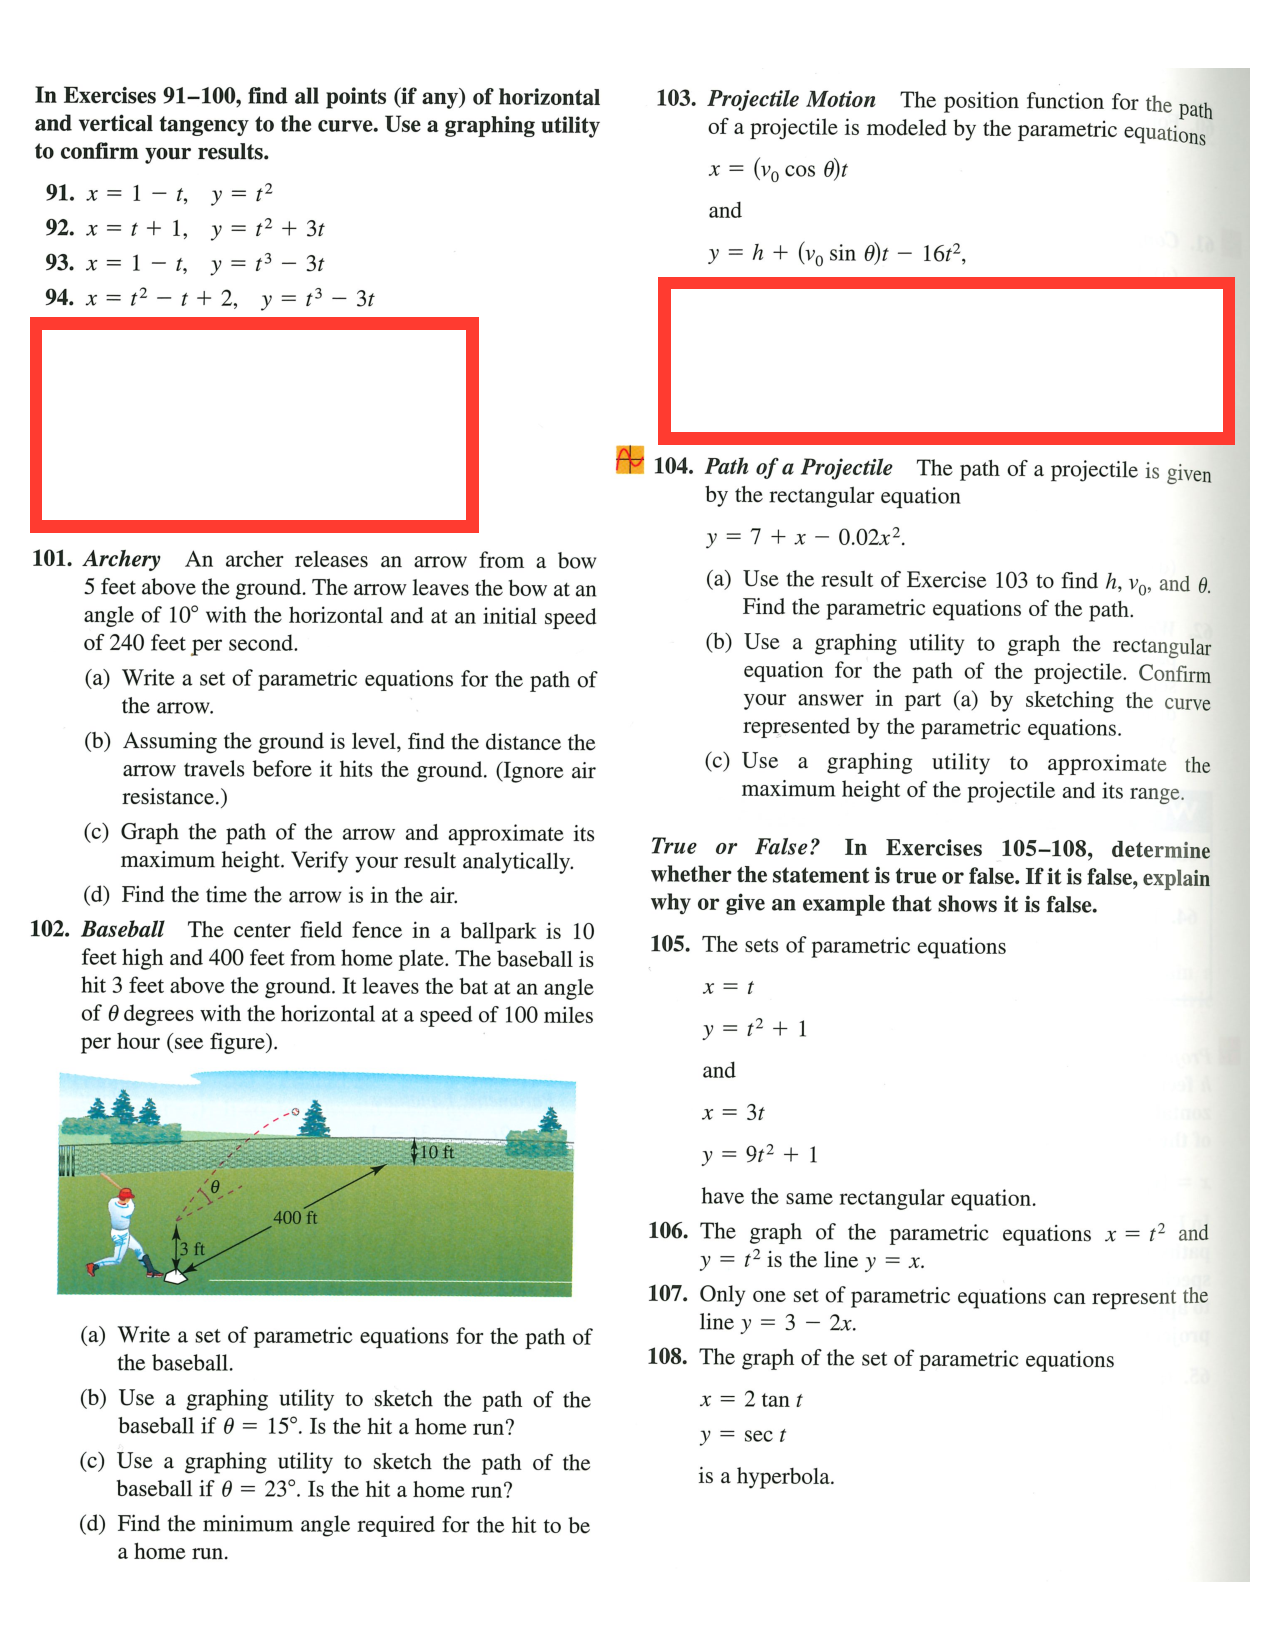
\includegraphics[width=\paperwidth]{ch04/0402xD.pdf}}



%							4 - 3
%\newpage
\invisiblesection{Composition}
%\subsection{Nesting}
\noindent\makebox[\textwidth]{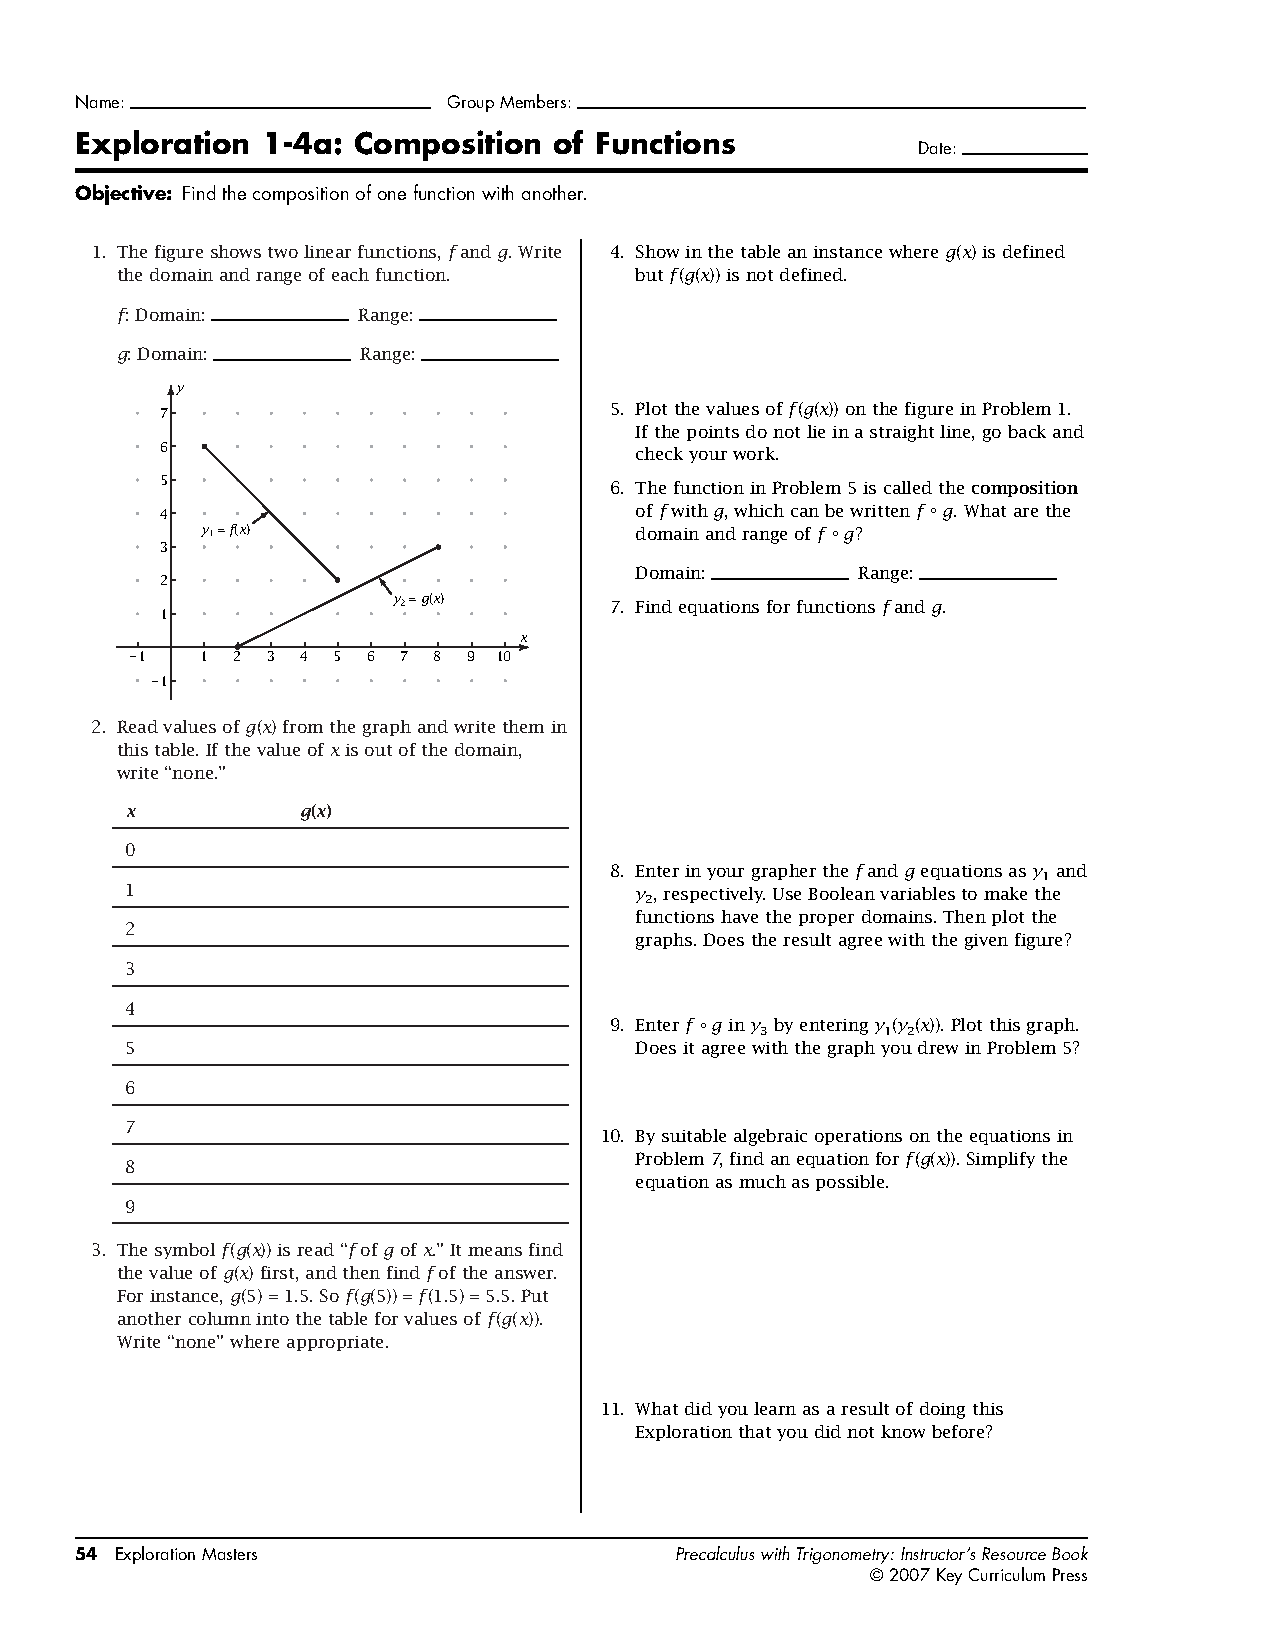
\includegraphics[width=\paperwidth]{ch04/0403p.pdf}}
\newpage
%!TEX root =  ../main.tex

\subsection{Pecking Order}

\objective{Build and decompose a composition of functions and their derivatives.}


In elementary school, we learned that a mathematics sentence has a 
certain order of operations, that somethings must happen before others.
If we want to add before we multiply, we must notate parentheses,
because normally multiplication is repeated addition, something of a higher
order than simple addition.  These parentheses lead to a phenomenon
in mathematics that is difficult and unnatural, compared to all other
languages: inside to outside reading.

For example, in the function $f(x)=\frac{2(x^2+1)}{3}$, you know to follow a
sequence of operations on any given input:
\begin{itemize}
\item square it
\item add 1
\item multiply by two
\item divide by three
\end{itemize}
Natural language does something like this, but it is quite confusing to read
(try saying it aloud to yourself): I saw the child the man my girl hates fathered.
It might be better to make this entirely left-branching: I saw the child who
the man fathered who my girl hates!

Our example utilizes only elementary functions: squaring, adding, multiplying,
and dividing.  If we want to use arbitrary functions, we must write
$f(g(h(x)))$ or $(f\circ g\circ h)(x)$.

\subsection{Domain and Range}
Taking a function as a composition of two other (e.g. $f(x)=g(h(x))$), we observe
a ``chain'' of inputs to outputs.  This might be compared to the game of telephone,
where your ear receives a message from the person before you, garbles it in your
brain, and then outputs a transformed version from your mouth, to the next person's
ear.  In math, there is a domain for $h(x)$, a set of numbers it can take for input.
These numbers are mapped onto a range of outputs, which are then fed into
$g(x)$.  Now $g(x)$ had its own domain, and the output from $h$ is a subset of that
absolute domain.  Having received some input from a portion of its domain,
$h(x)$, now outputs a unique range.

\begin{figure}
\begin{center}
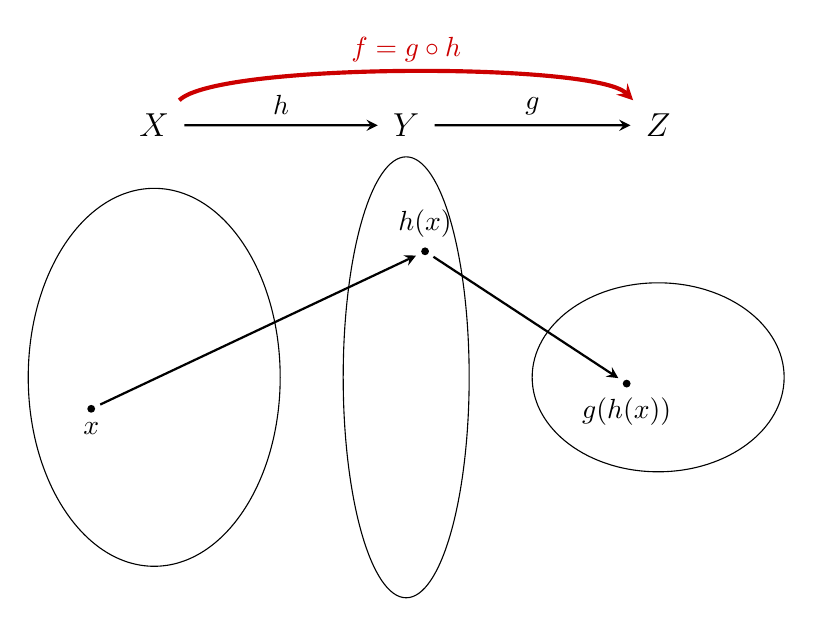
\begin{tikzpicture}[scale=0.8,
      >=stealth,
      bullet/.style={
        fill=black,
        circle,
        inner sep=1pt
      },
      projection/.style={
        ->,
        thick,
        shorten <=2pt,
        shorten >=2pt
      },
    ]

    \draw (0, 0) circle [x radius=2, y radius=3];
    \node [bullet, label=below:\(x\)] (x) at (-1, -0.5) {};
    \node[font=\large] (X) at (0, 4) {\(X\)};

    \begin{scope}[xshift=4cm]
      \draw (0, 0) circle [x radius=1, y radius=3.5]; \node [bullet,
      label=above:\(h(x)\)] (fx) at (0.3, 2) {};
      \node[font=\large] (Y) at (0, 4) {\(Y\)};
    \end{scope}
    \begin{scope}[xshift=8cm]
      \draw (0, 0) circle [x radius=2, y radius=1.5]; \node [bullet,
      label=below:\(g(h(x))\)] (gfx) at (-0.5, -0.1) {};
      \node[font=\large] (Z) at (0, 4) {\(Z\)};
    \end{scope}

    \draw [projection] (x) -- (fx);
    \draw [projection] (fx) -- (gfx);
    \draw [projection] (X) -- (Y)
          node [pos=0.5, above] {\(h\)};
    \draw [projection] (Y) -- (Z)
          node [pos=0.5, above] {\(g\)};
    \draw [out=45, in=180-45, projection, line width=1.5pt, red!80!black] 
          (X) .. controls ++(1, 1) and ++(-1, 1) .. (Z)
          node [pos=0.5, above] {\(f = g \circ h\)};
\end{tikzpicture}
\caption{Composition of functions \cite{sxtikzcomp}.}
\end{center}
\end{figure}
  
\subsection{Decomposition}
Any function with more than one operation can be written as the composition of
other functions.  For example, if $f(x)=x^2+1$ then we could construct
functions $g(x)=x^2$ and $h(x)=x+1$ such that $f(x)=h(g(x))$ ($g(h(x))$ would be
$(x+1)^2$).

\subsection{The Chain Rule}\index{derivative!chain rule}
The algebra of functions continues, even into the realm of derivatives.  Two functions
added would have a simple derivative: the sum of their respective derivatives.  But what 
of two functions composed?  What is the derivative of $g(h(x))$?

Here, Leibniz's notation is more helpful:

$$f(x)=g(h(x)), \quad \frac{df}{dx}=\frac{dg}{dh}\cdot\frac{dh}{dx}$$

\paragraph{Trigonometric Derivatives}\index{derivative!of sine}
While you are not responsible for proving and understanding trigonometric functions
until Part~\ref{pt:trig}, it is helpful to being memorizing facts about them now.  This will allow
you to practice manipulating the functions like any other.  However, to do so, you will
need to know the derivative of sine and cosine.\index{derivative!of cosine}

\begin{itemize}
\item $f(x) = \sin(x)$
\item $f'(x) = \cos(x)$
\item $f''(x) = -\sin(x)$
\item $f'''(x) = -\cos(x)$
\item $f^{(4)}(x) = \sin(x)$
\end{itemize}
As you can see, a straightforward, four-step cycle emerges.  The derivative of sine is
cosine.  The derivative of cosine is negative sine.



\newpage
\subsection{Exercises}
\noindent\makebox[\textwidth]{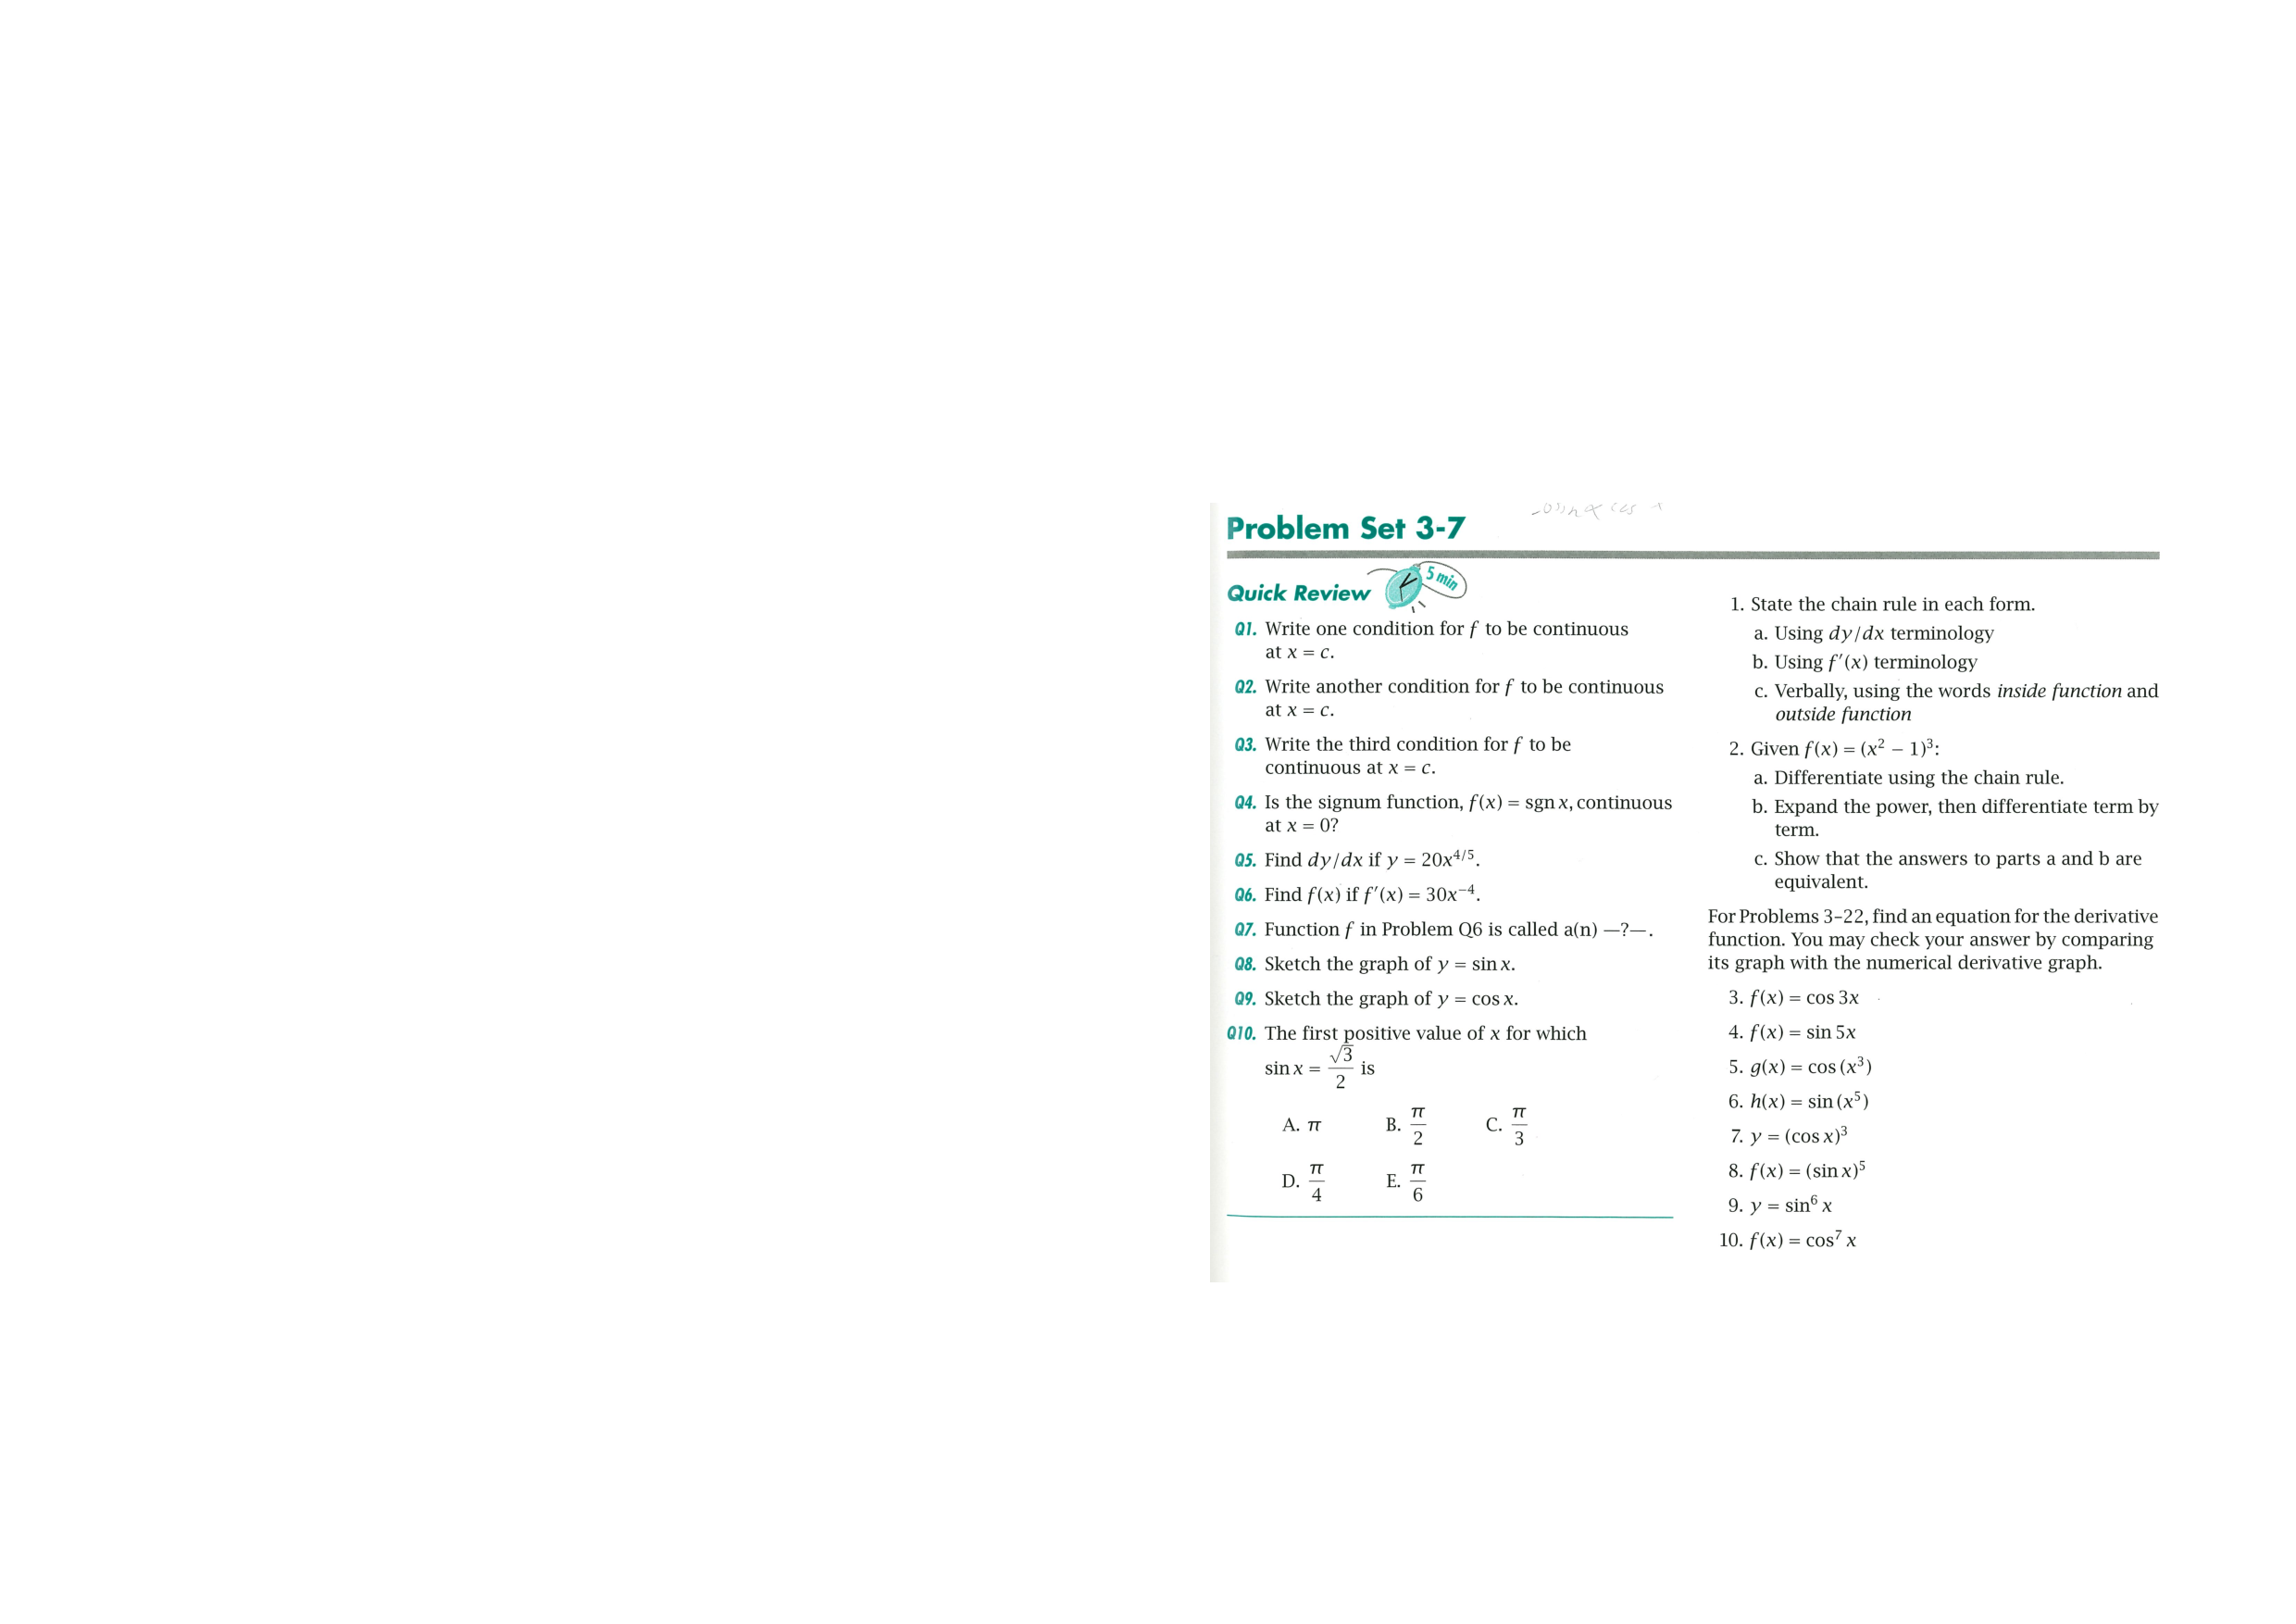
\includegraphics[width=\paperwidth]{ch04/0403xA.pdf}}
\newpage
\noindent\makebox[\textwidth]{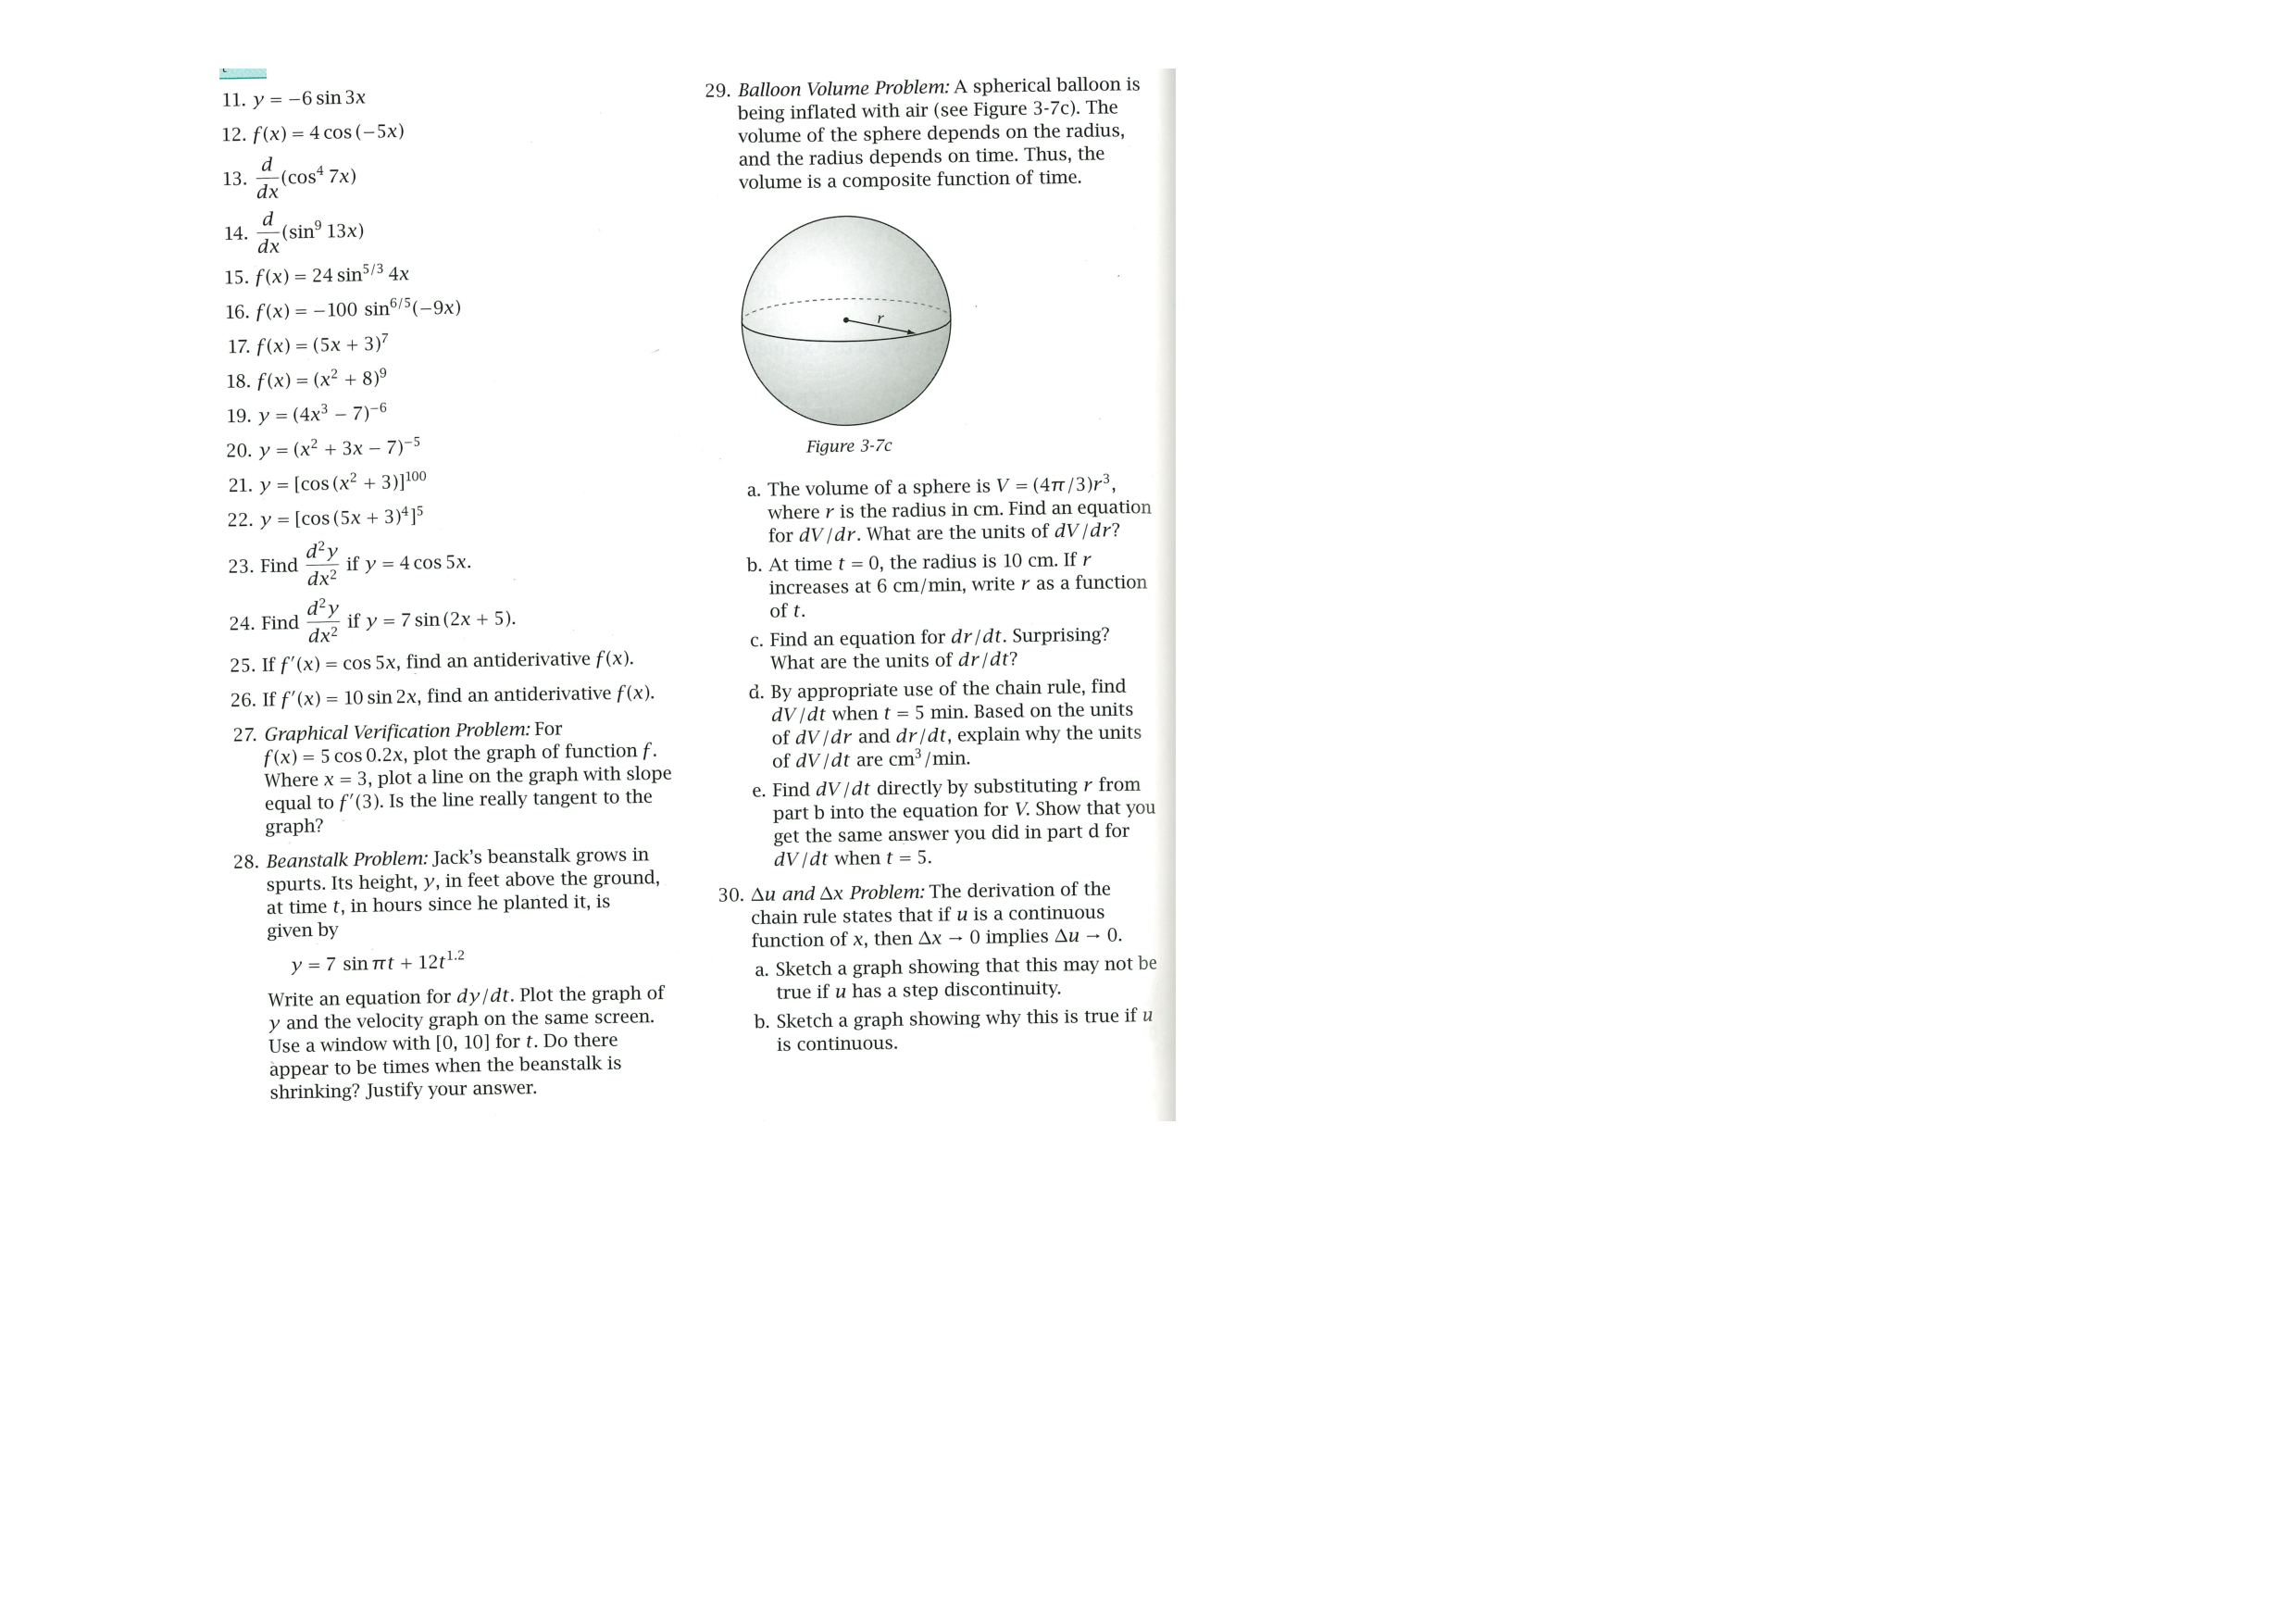
\includegraphics[width=\paperwidth]{ch04/0403xB.pdf}}
\newpage
\noindent\makebox[\textwidth]{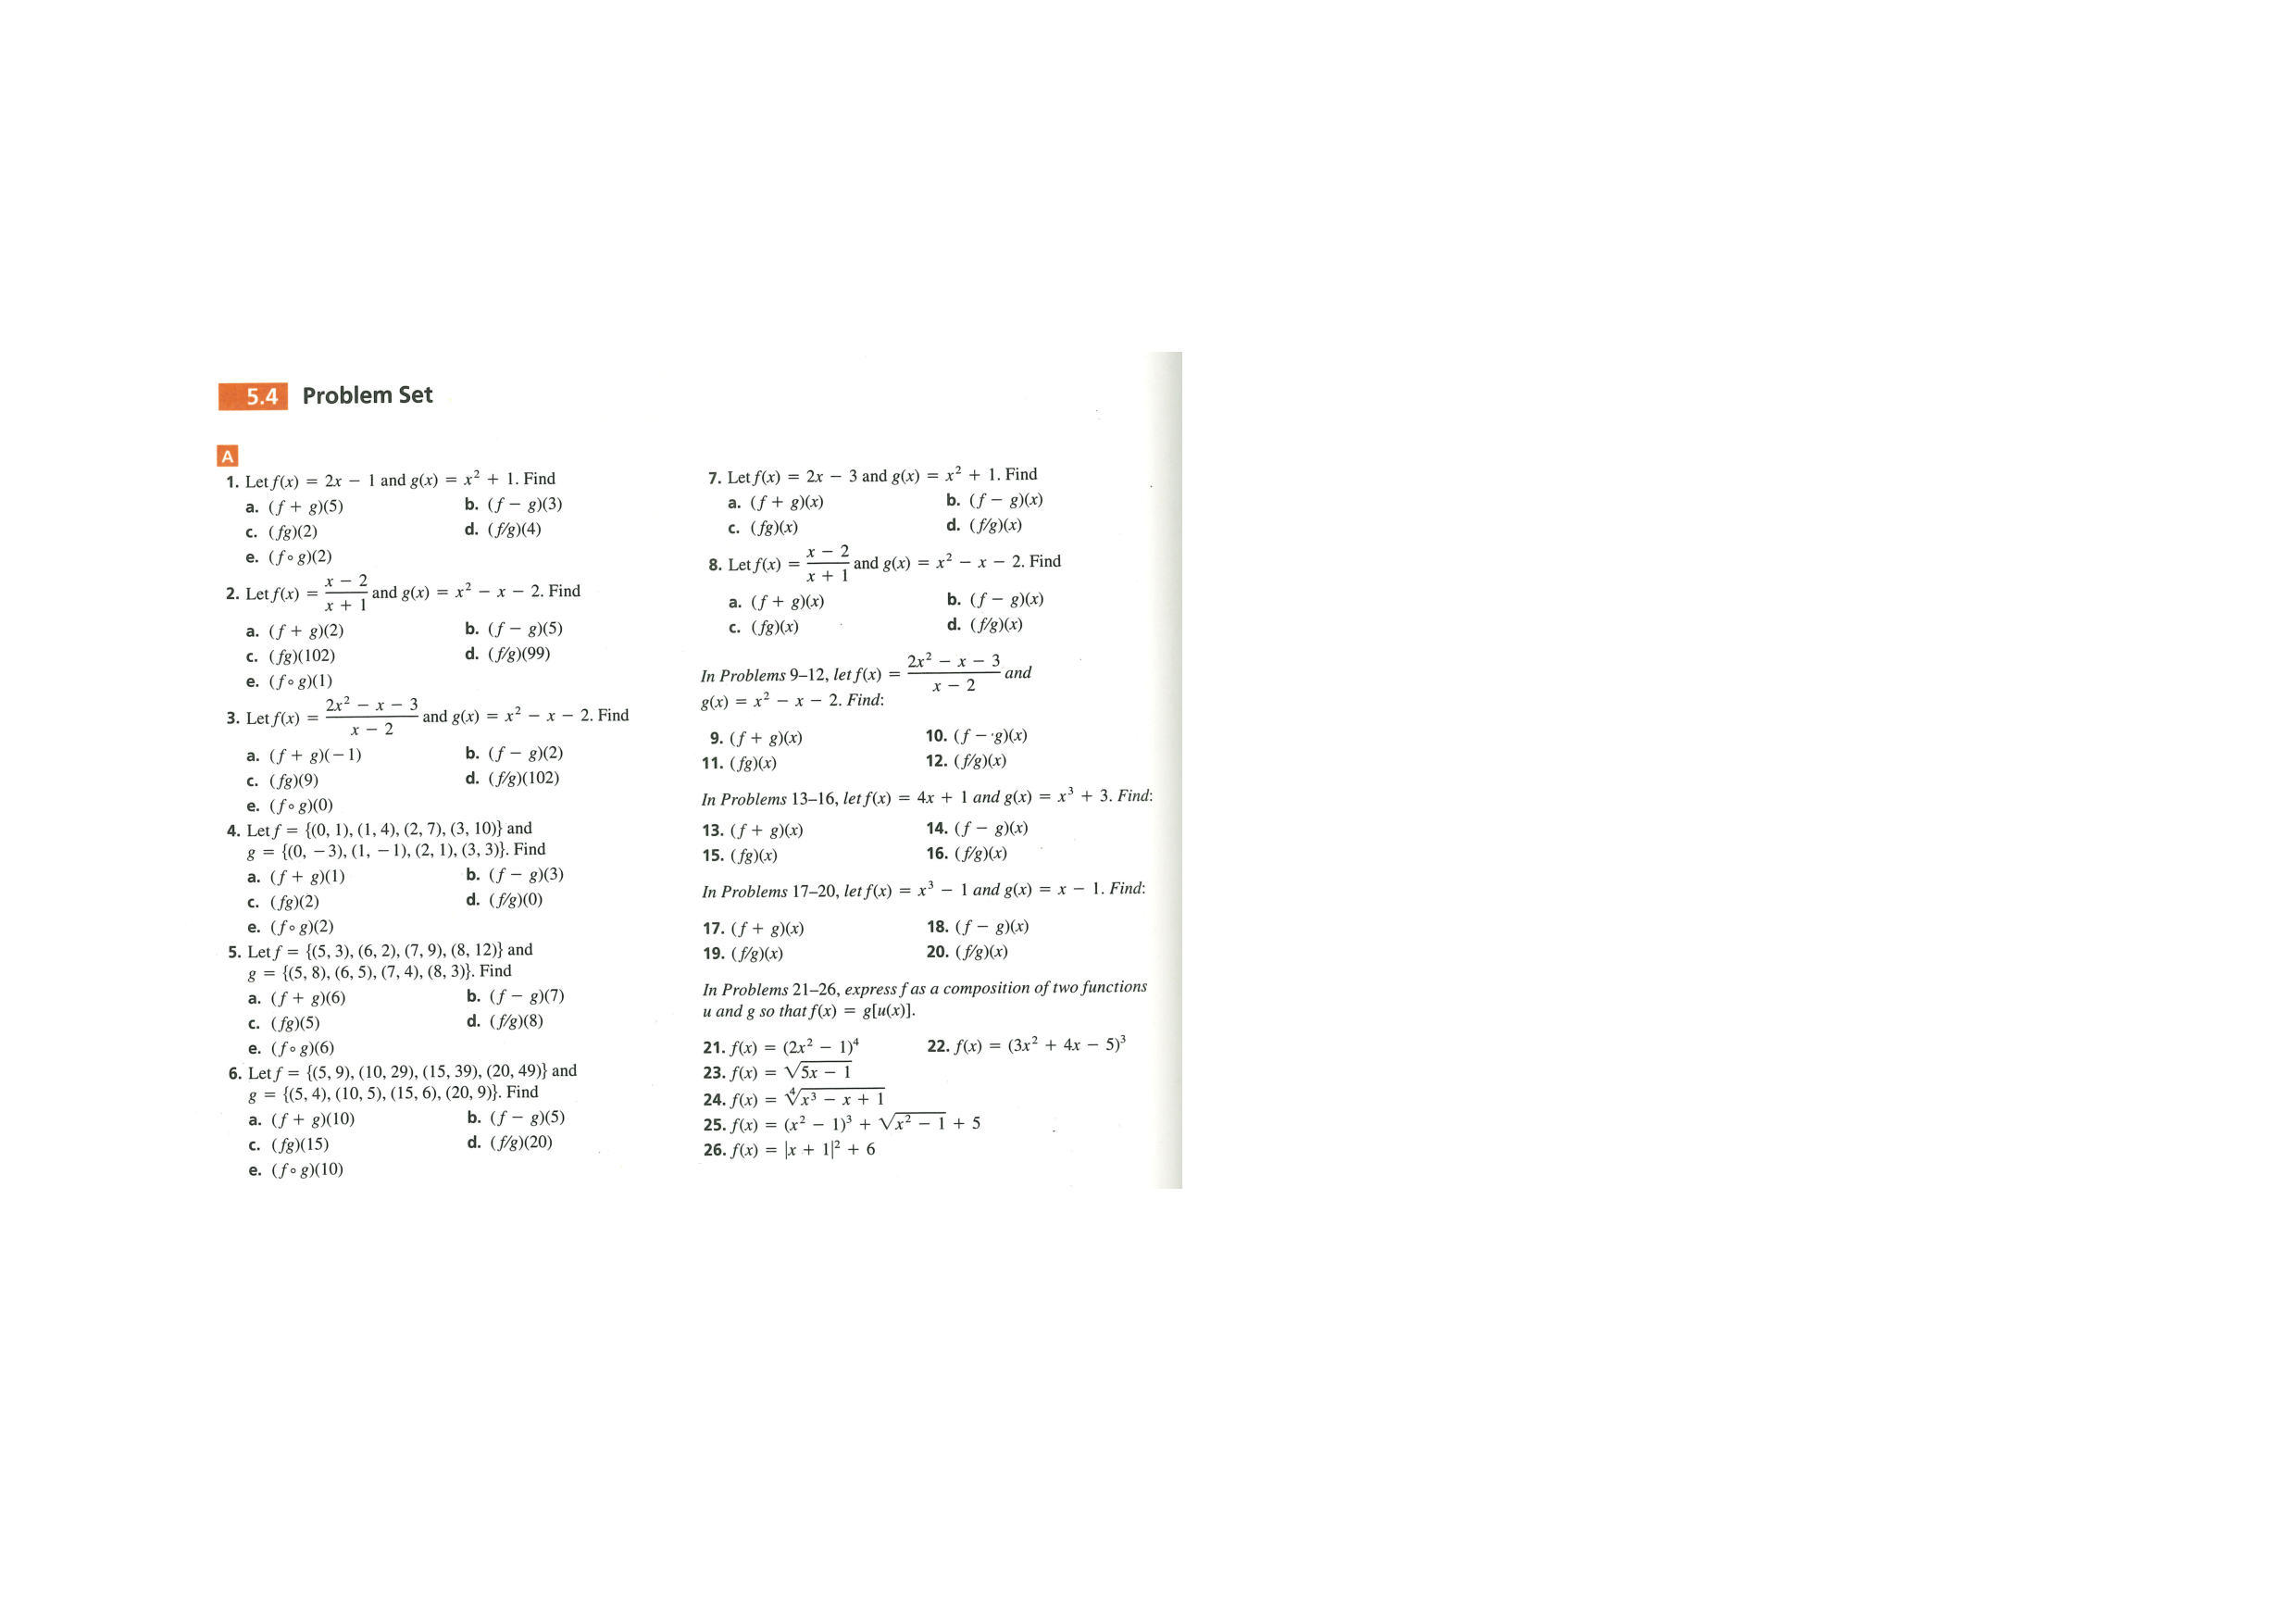
\includegraphics[width=\paperwidth]{ch04/0403xC.pdf}}
\newpage
\noindent\makebox[\textwidth]{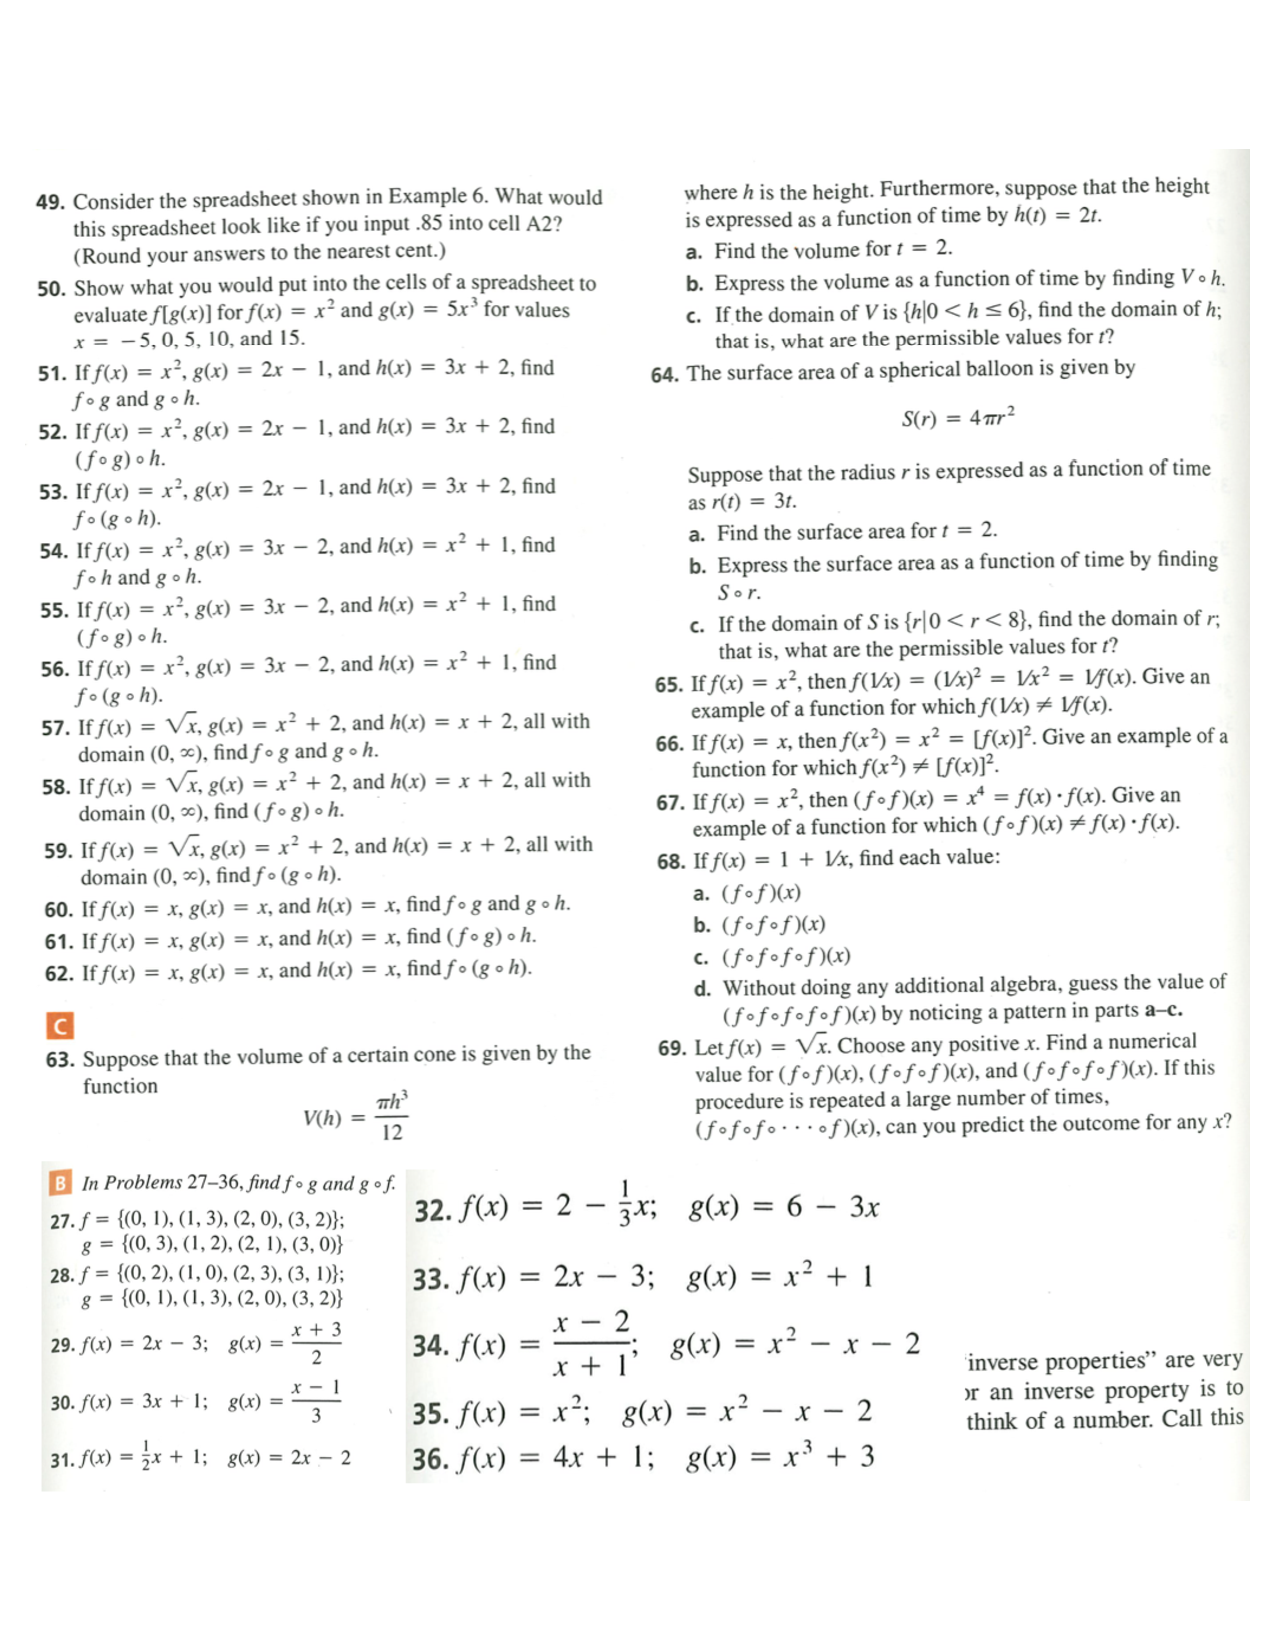
\includegraphics[width=\paperwidth]{ch04/0403xD.pdf}}



%							4 - 4
\newpage
\section{Reciprocal}
\subsection{``Upside Down''}
made in Word
\newpage
%!TEX root =  ../main.tex

\subsection{Numerically}

\objective{Calculate and graph reciprocal functions.}

Calculating the reciprocal of a function is very straightforward.  For any given $x$,
take the output $f(x)$, and then reciprocate that number.  What that leads to is a
complicated picture.  However, a pattern emerges.  The reciprocal of 1 is 1, and the
reciprocal of -1 is -1.  That means points on the graph with a $y$ of 1 will not
be effected by reciprocation.  Other integer outputs will reciprocate to smaller and
smaller fractions, e.g. 2 to $\frac{1}{2}$, 3 to $\frac{1}{3}$, etc.

What is unusual is the behavior around 0.  Zero has no reciprocal, so there will 
typically be a vertical asymptote.

Especially in trigonometry, reciprocals can have names.

\begin{figure}
\begin{centering}
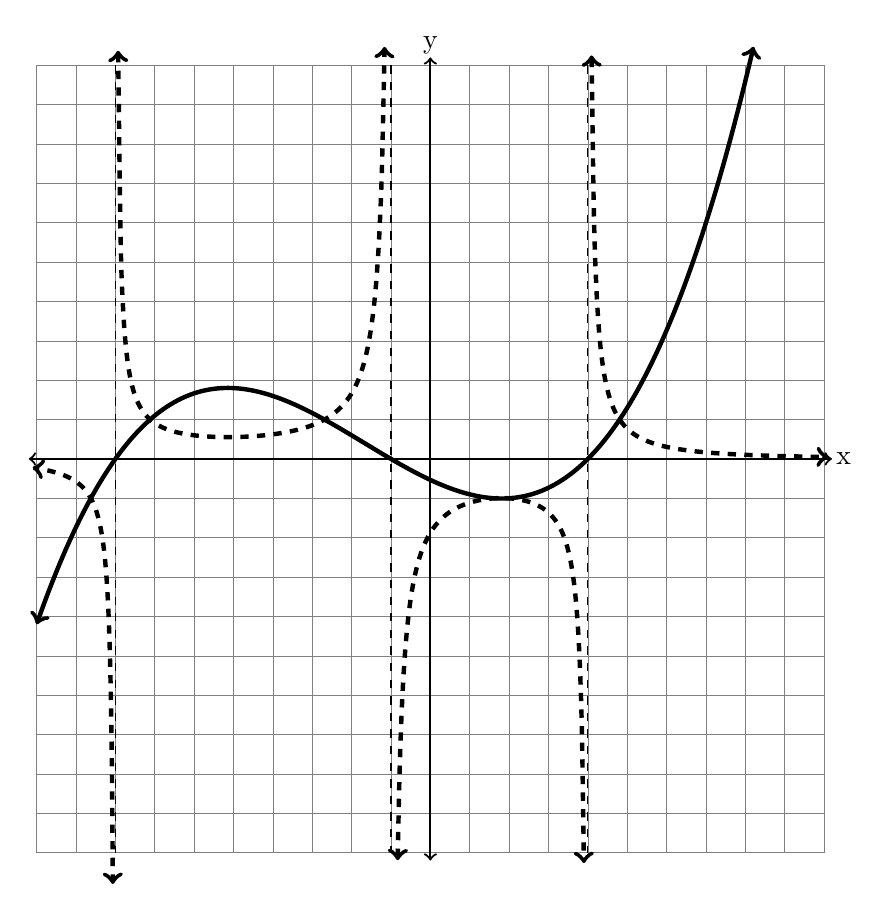
\begin{tikzpicture}[scale=0.5]
	\draw [help lines] (-10, -10) grid (10, 10);
	\draw [thick,<->] (-10.2, 0) -- (10.2, 0);
	\draw [thick,<->] (0, -10.2) -- (0, 10.2);
        % x-axis label
        \node at (10.5, 0) {x};
        % y-axis label
        \node at (0, 10.5) {y};
        \draw[domain=-10:8.21,<->,ultra thick,samples=100,smooth] plot (\x,{1/60*(\x-4)*(\x+1)*(\x+8)});
        \draw[domain=-10.1:-8.065,<->,ultra thick,samples=100,smooth,dashed] plot (\x,{60/((\x-4)*(\x+1)*(\x+8))});
        \draw[domain=-7.93:-1.162,<->,ultra thick,samples=100,smooth,dashed] plot (\x,{60/((\x-4)*(\x+1)*(\x+8))});
        \draw[domain=-.83:3.9,<->,ultra thick,samples=100,smooth,dashed] plot (\x,{60/((\x-4)*(\x+1)*(\x+8))});
        \draw[domain=4.095:10.1,<->,ultra thick,samples=100,smooth,dashed] plot (\x,{60/((\x-4)*(\x+1)*(\x+8))});
        \draw[dashed, -] (-1,10) -- (-1,-10);
        \draw[dashed, -] (-8,10) -- (-8,-10);
        \draw[dashed, -] (4,10) -- (4,-10);
\end{tikzpicture}
\caption[Example of graphical reciprocation]{An example of a function and its reciprocal, $f(x)=\frac{1}{60}(x-4)(x+1)(x+8)$.}
\end{centering}
\end{figure}
~\vfill
\newpage
\subsection{Exercises}
Word, needs circle inversion geometry
~\vfill


%							4 - 5
%\newpage
\invisiblesection{Inverse}
\noindent\makebox[\textwidth]{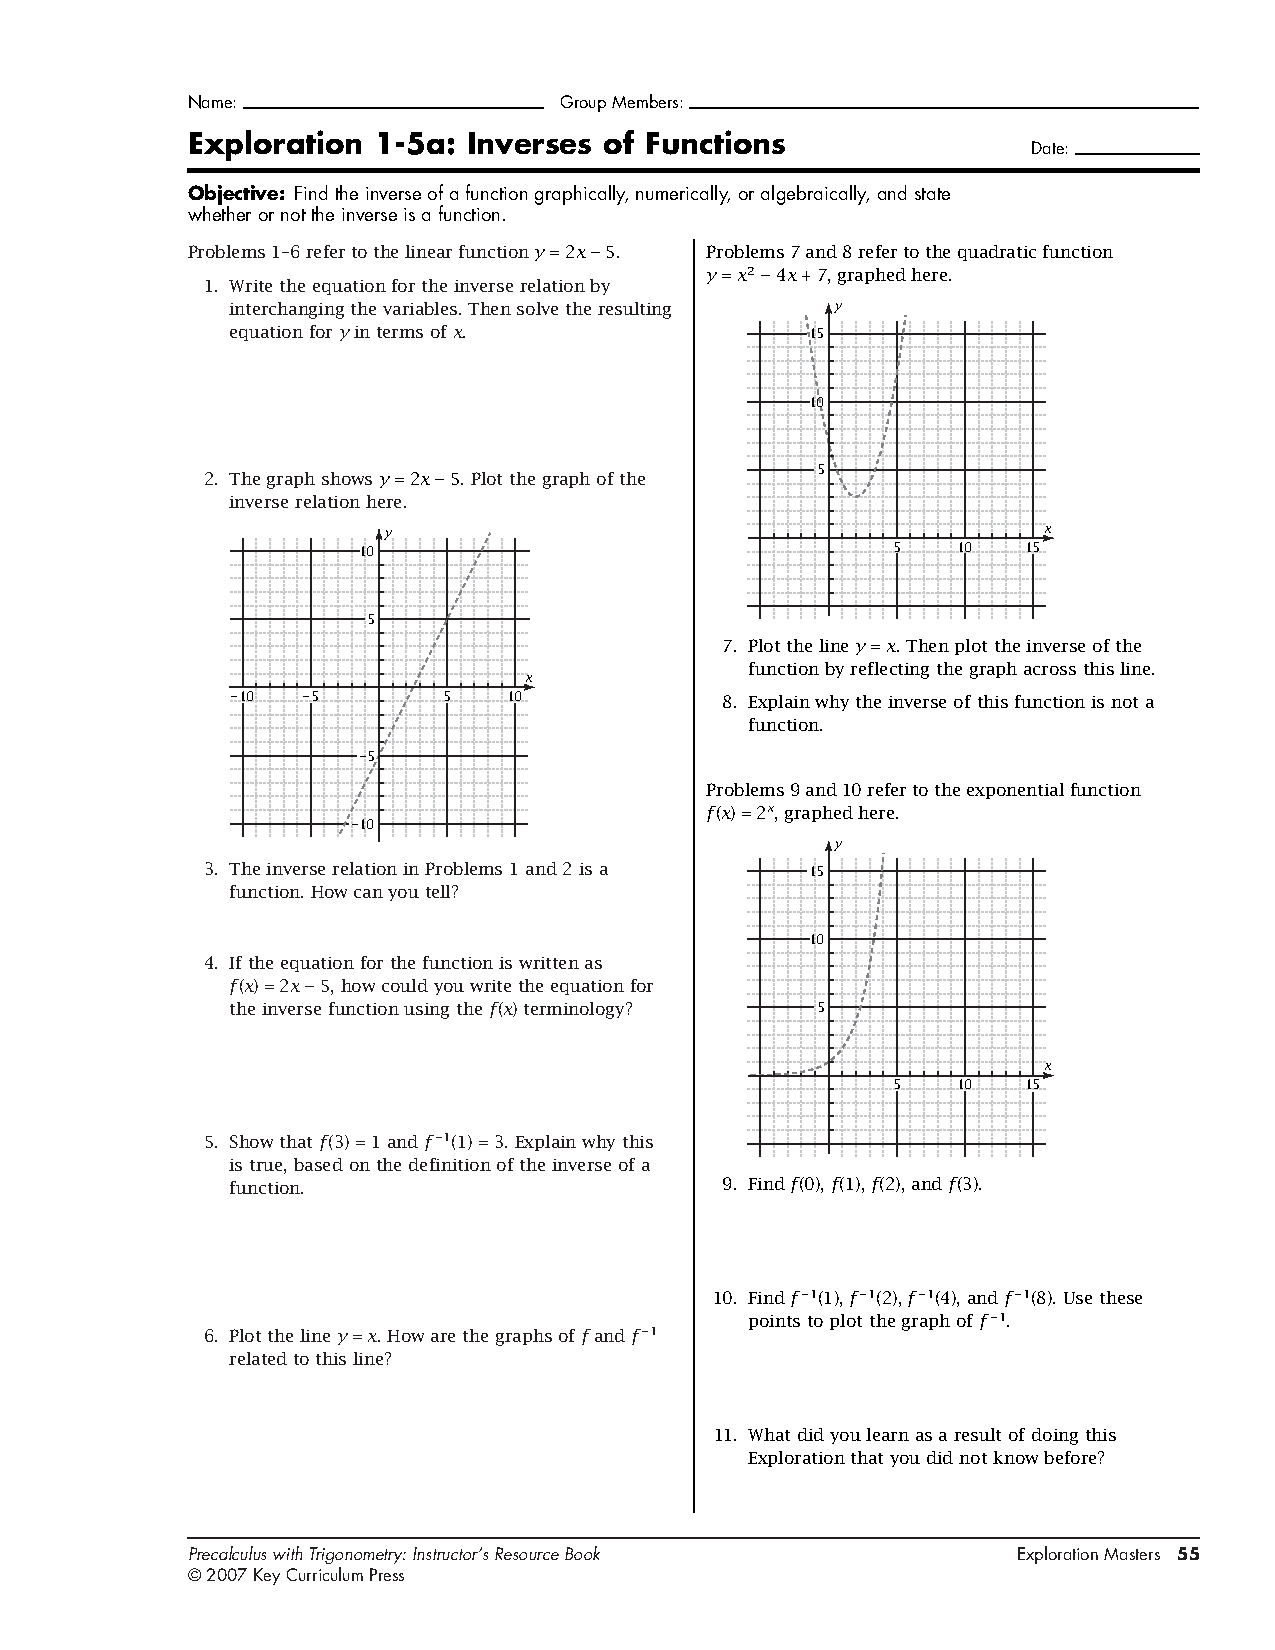
\includegraphics[width=\paperwidth]{ch04/0405p.pdf}}
%!TEX root =  ../main.tex

\subsection{``Undo''}

\objective{Find and graph function inverses and their derivatives.}


We have seen that functions can be redefined as the composition of other, simpler
functions.  For example, $\frac{x^2+1}{2}$ can be seen as 1) squaring, 2) adding 1
, and 3) dividing by 2.  What if we wanted to ``undo'' the effects of this function?
We cannot simply do the opposite of each operation ($\frac{\sqrt{x} -1}{2}$ is not
the inverse) but must do the opposites \emph{backwards}.  This is called the
\textbf{inverse} of the function.  

\subsection{Swap $x$ and $y$}
In the example already mentioned, the inverse is $\pm\sqrt{2x-1}$.  What is wrong with 
this inverse?  It is not a function.  No even power has an inverse which is a function, because
there are infinitely many places where a particular output is reached from two different inputs.
Another way to think of inverses is reversing $x$ and $y$, making the output the input and
visa versa.  Only \textbf{one-to-one} functions --- where every $x$ has a \emph{unique}
$y$ --- will have inverses which are themselves functions.

Numerically, this shows how easy it is to construct an inverse of data: simply swap the
column labels for input and output!   This can be done algebraically too.  Staying with
the same example, we could follow the procedure of 1) swapping $x$ and $y$, and then
2) solving for $y$ to find the inverse of a function.

\begin{align*}
	y &= (x^2+1)/2 \\
	x &= (y^2+1)/2\\
	2x &= y^2+1\\
	2x - 1 &= y^2 \\
	\pm\sqrt{2x-1} &= y\\
\end{align*}

\subsection{S.I.F.T.}
But such examples fail when there are multiple places where $x$ appears in the equation
of $y$.  How can we find the inverse of $y=\sqrt{\frac{x-1}{2-x}}$  A helpful acronym to 
remember is such cases is S.I.F.T., which standard for
\begin{itemize}
\item[\textbf{S}pread] Clear the fractions, exponentiate the roots away, distribute the parentheses, etc.
\item[\textbf{I}solate] Move all the terms with the desired variable onto one side of the equation, and move all the other terms to the opposite side.
\item[\textbf{F}actor] Factor out the desired variable from all the terms on its side
\item[\textbf{T}ransfer] Divide off the term in parentheses, leaving the variable alone.
\end{itemize}
Returning to our hard example:

\begin{align*}
	y  &= \sqrt{\frac{x-1}{2-x}}\\
	x  &= \sqrt{\frac{y-1}{2-y}}\\
	x^2 &= \frac{y-1}{2-y}\\
	x^2(2-y) &= y-1 \\
	2x^2-x^2y &= y-1 &\text{finally spread out}\\
	2x^2 + 1 &= y + x^2y & \text{$y$ is isolated on the right}\\
	2x^2 + 1 &= y(1+x^2) & \text{factored out $y$}\\
	\frac{2x^2+1}{1+x^2} &= y & \text{transferred}
\end{align*}


\subsection{Graphically}
Inverses --- whether they are a function or not --- are a reflection across the line $y=x$.
This leads to some amazing properties of there derivatives.

Consider the function $f(x) = (x-1)^3+4$, a simple cubic function, shift right 1 and up 4.
It's derivative is easy to calculate: $f'(x)=3(x-1)^2$.  It's inverse somewhat more complicated,
but perhaps it is enough to sketch it, swapping $x$ and $y$ at every point, reflecting it over
the line $y=x$.

\begin{figure}[h]
\begin{centering}
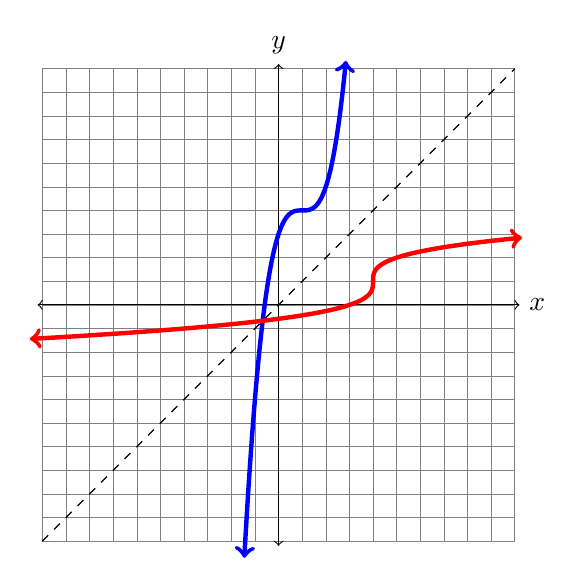
\begin{tikzpicture}[scale=0.3]
\draw[help lines] (-10,-10) grid (10,10);
\draw[<->] (-10.2,0) -- (10.2,0) node[anchor=west] {$x$};
\draw[<->] (0,-10.2) -- (0,10.2) node[anchor=south] {$y$};
\draw[dashed] (-10,-10) -- (10,10);
\draw[domain=-1.45:2.85,ultra thick,<->,samples=200,smooth,blue] plot (\x,{(\x-1)^3+4});
\draw[<->,domain=-1.44:2.85,samples=200,smooth,red,ultra thick]plot({(\x-1)*(\x-1)*(\x-1)+4},\x);
\end{tikzpicture}
\caption[Graphical example of inverses]{A function and its inverse, which are clearly reflections of each other across the line $y=x$.}
\end{centering}
\end{figure}

This can be done easily on the TI-8*.   First, enter the original function in $Y_1$ and graph
it.  Be sire you have a window appropriate to the function and it's inverse!  Next, select DRAW
and choose option 8: DrawInv, passing it the argument $Y_1$.  Press ENTER and 
you will be able to see the inverse.  Unfortunately, we cannot TRACE along it or any of the 
other tools we are used to for functions, but that hardly matters.  

Consider the tangent line through (2,5) on the original graph.  Hopefully, it is easy for
you to calculate that it follows the equation $y-5=3(x-2)$.  Enter this as $Y_2$.
Have the TI-8* draw its inverse.  This second line will pass through the point (5,2)
and have a reciprocal slope: $\frac{1}{3}$.

This shows that the derivative of the inverse is equal to the reciprocal of the derivate,
for every point $(x,y)$ which has been mapped onto $(y,x)$.
\index{derivative!of the inverse}

\newpage
\subsection{Exercises}
\noindent\makebox[\textwidth]{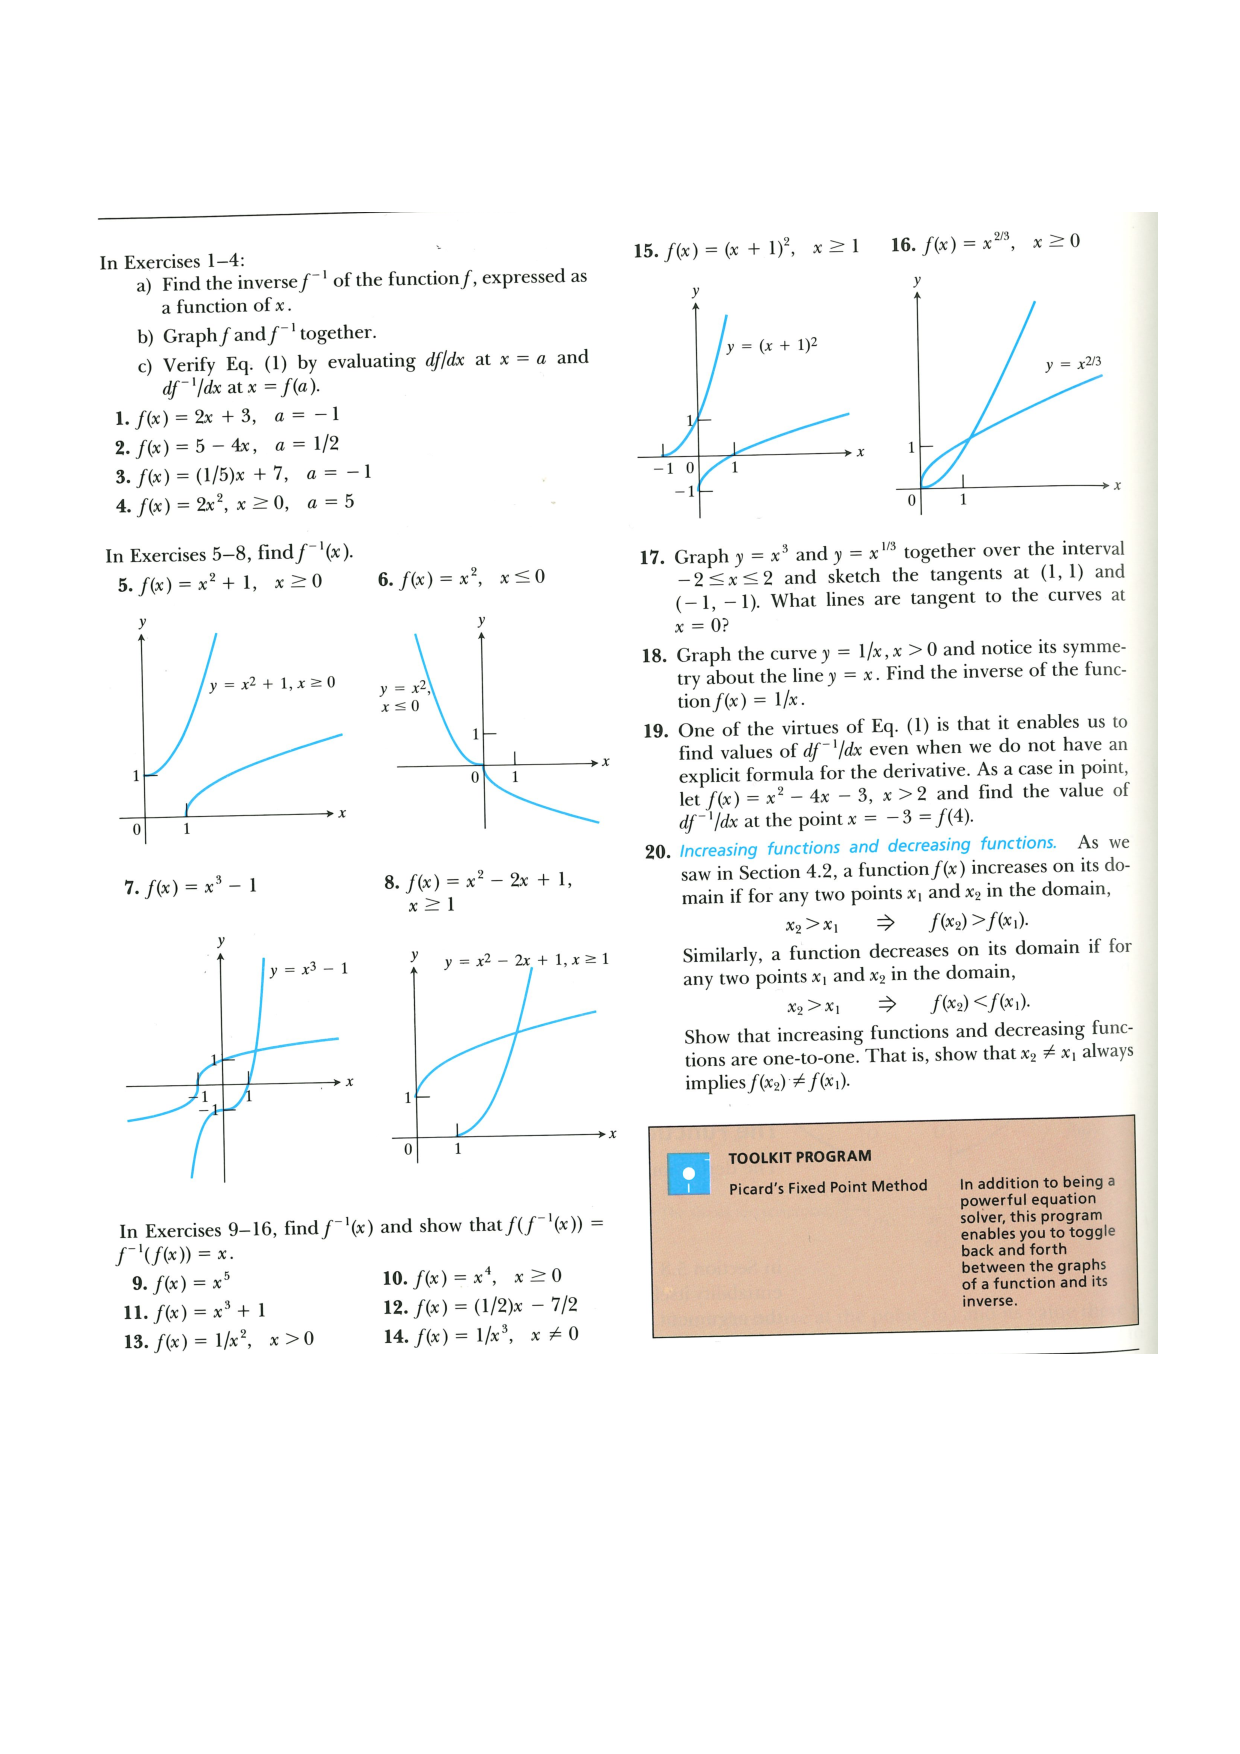
\includegraphics[width=\paperwidth]{ch04/0405x.pdf}}




\newpage
\section{Review}
\subsection{Chapter Review}
In this chapter we saw that the absolute value of common quantities have names and that absolute
values of known functions are reflections of certain parts of the graph only.  
A function does not have to mean $y$ is a function of $x$: they can both be a function of
another variable, usually time.  Another way to write the derivative is $\frac{dy}{dx}$.
We saw that most functions can be understood as being
made out of parts --- called composition.  The rate of change of such these ``Russian doll''
functions is ``the derivative of the outside times the derivative of the inside''.

Next we looked at the reciprocals of graphs and lastly the inverses.  With numbers, these can
be notated the same way, but with functions, there is no shortcut to writing the derivative.
An inverse is the ``undo'' of a function, the swapping of input for output.  However, not all 
functions are reversible across their entire domain.  The derivative of the inverse if the same
as the reciprocal of the derivative.

\subsection{Chapter Test}
\subsection{Cumulative Review} 
This major section of the book has been about algebraic functions, that is, functions made out
of addition, subtraction, multiplication, division, and exponents (roots are exponents).  We 
can either evaluate a function at a point, or take its limit.  Functions can be manipulate
algebraically or even combined.  We can move fluidly from verbal to numeric to algebraic to
graphical, or any combination thereof.  Algebraic functions have algebraic derivatives and are
themselves derivatives of more algebraic functions.
\subsection{Cumulative Test}
